\documentclass{rnu-thesis}

\usepackage[protrusion]{microtype}

\usepackage{makecell}
\renewcommand{\arraystretch}{1.2}

% --- Algorithms (kept for template compatibility, no algorithms used in this thesis)
\usepackage{algorithm}
\usepackage{algpseudocode}
\usepackage{float}

% --- TikZ for diagrams
\usepackage{tikz}
\usetikzlibrary{arrows.meta,positioning,shapes.geometric,shapes.symbols,fit,calc,matrix,graphs}
\tikzset{>=Stealth}

% --- pgfplots for charts
\usepackage{pgfplots}
\pgfplotsset{compat=1.18}


% --- Code listings
\usepackage{listings}
\usepackage{xcolor}
\lstset{
  basicstyle=\ttfamily\small,
  numbers=left,
  numbersep=6pt,
  frame=single,
  breaklines=true,
  tabsize=2,
  showstringspaces=false,
  float=htbp,
  captionpos=t
}

% --- Bibliography via biblatex (IEEE numeric)
\usepackage[backend=biber,style=ieee,sorting=nty,maxbibnames=99]{biblatex}
\addbibresource{x_bibliography/references.bib}
\nocite{*}


% ====== Thesis info ======
\setthesisinfoLV
  {M\=akslīg\=a intelekta Telegram bota izstr\=ade person\-aliz\=etiem d\=avanu ieteikumiem, izmantojot prompt in\v zen\-ierijas tehnikas}% LV Title
  {Samandar Olimov}% LV Student
  {Dr.sc.ing., Professor, Jelena Caiko}% LV Supervisor
  {42484 Inform\=acijas sist\=emas (bak.)}% LV Programme
  {Dabaszin\=at\c nu un dator\-teh\-no\-lo\-\v gi\-ju katedra}% LV Department
  {2026}% Year

\setthesisinfoEN
  {Development of an AI-Powered Telegram Bot for Personalized Gift Recommendations Using Prompt Engineering Techniques}% EN Title
  {Samandar Olimov}% EN Student
  {Dr.sc.ing., Professor, Jelena Caiko}% EN Supervisor
  {42484 Information Systems (BSc)}% EN Programme
  {Department of Natural Sciences and Computer Engineering}% EN Department
  {2026}% Year

% ====== Scope - count manually before final submission ======
\setthesisscope
  {55}% Total pages (estimate; recount final PDF)
  {14}% Total tables
  {7}% Total figures
  {0}% Total algorithms
  {11}% Total listings
  {3}% Total annexes (A, B, C)
  {22}% Total references
\begin{document}

\input{a_frontmatter/title_page_lv}
\clearpage
\input{a_frontmatter/title_page_en}
\clearpage

\pagenumbering{arabic}

% ===== Abstracts & Keywords =====
\chapter*{Anot\=acija (LV)}
\addcontentsline{toc}{chapter}{Anot\=acija (LV)}

\textbf{Nosaukums:} M\=ak\-sl\=ig\=a intelekta Telegram bota izstr\=ade person\-aliz\=etiem d\=avanu ieteikumiem, izman\-tojot prompt inženierijas tehnikas.

D\=avanas izv\=ele ir ikdienišks, bet laikietilp\=igs uz\-de\-vums. Tieš\-saistes veikali r\=ada daudz pre\-\v cu, bet ne\-pied\=av\=a person\-aliz\=etus padomus. Mo\-derni lielie va\-lo\-das mode\-\c li (LLM) var ana\-liz\=et d\=avanas sa\-\c n\=em\=eja profilu un ie\-te\-ikt da\-v\=anu ide\-jas da\-bisk\=a va\-lo\-d\=a. Ta\-\v cu LLM at\-bilžu kva\-lit\=ate ir \c lo\-ti at\-ka\-r\=iga no ievades teksta (prompta) di\-zaina. Šo problē\-mu p\=et\=i jauna pē\-t\=ij\=umu jo\-ma — prompt in\-žen\-ierija.

Darba m\=er\c kis ir iz\-strā\-d\=at Tele\-gram botu, kas iz\-manto LLM (Grok no xAI), lai sniegtu person\-aliz\=etus d\=avanu iete\-ikumus, un sa\-l\=id\-zin\=at \v cetras prompt in\v zen\-ierijas stra\-t\=e\-\v gi\-jas šim uz\-de\-vu\-mam: Naive, Cons\-trai\-ned, Chain-of-Thought (CoT) un Per\-sona-based.

Bots tika izstr\=ad\=ats Python valod\=a, izmantojot aiogram bibliot\=eku un SQLite datu b\=azi. Lieto\-t\=ajs iziet \=isu anketu ar sešiem strukturi\-z\=etiem jaut\=ajumiem un sa\-\c nem trīs personaliz\=etas d\=avanu idejas. Sis\-t\=ema ir izvietota PythonAnywhere m\=ako\-\c na pla\-tform\=a.

Tika veikts kontrol\=ets eksperiments. Tika sagatavotas 30 sin\-t\=etiskas lietot\=aju per\-sonas. Visas \v cetras stra\-t\=e\-\v gi\-jas tika izpild\=itas uz vis\=am person\=am, kop\=a — 120 testa gad\=ijumi. Katra atbilde tika nov\=ert\=eta p\=ec piec\=am metrik\=am: re\-le\-vance, ra\-doš\=ums, specifis\-kums, halluci\-n\=acijas iezīme un at\-bildes laiks. Bots tika test\=ets ar\=i ar 8 re\=alajiem lietot\=ajiem.

Rezult\=ati apstiprina hipot\=ezi, ka uzlabot\=as stra\-t\=e\-\v gi\-jas dod ie\-v\=ero\-jami labākus iete\-ikumus nek\=a vienkārš\=a (naive) pieeja. Lab\=ak\=a kop\=ej\=a stra\-t\=e\-\v gi\-ja bija Chain-of-Thought (relevance 4.43/5, hallucin\=acija 8.9\%). Visradoš\=ak\=a stra\-t\=e\-\v gi\-ja bija Persona-based (radoš\=ums 4.53/5). Visas \v cetras stra\-t\=e\-\v gi\-jas atbild\=eja mazāk nek\=a 10 sekund\=es. 75\% lietot\=aju teica, ka izmantotu botu atk\=al.

Darb\=a ir pied\=av\=ati turp\-m\=akie uzla\-bo\-jumi: integr\=acija ar p\=ardošanas platform\=am, daudz\-mod\=ala ievade, daudzva\-lod\=u atbalsts un hib\-r\=id\=a prompt pipeline.

Darbs ap\-stiprina, ka prompt in\-žen\-ierija ir re\=ala un izm\=erojama in\-žen\-ierijas dar\-b\=iba. Pied\=av\=at\=a meto\-do\-lo\-\v gi\-ja ir do\-m\=ena ne\-at\-ka\-r\=iga un to var izmantot citos personaliz\=etos rekomend\=aciju uzde\-vumos.

\textbf{Apj\=oms:} 55 lappuses, 14 tabulas, 7 at\-tē\-li, zx atsauces, 22 pielikumi.

\chapter*{Abstract (EN)}
\addcontentsline{toc}{chapter}{Abstract (EN)}

\textbf{Title:} Development of an AI-Powered Telegram Bot for Personalized Gift Recommendations Using Prompt Engineering Techniques.

Choosing a gift is a common but time-consuming task in daily life. Online marketplaces show many products but no personalized advice. Modern Large Language Models (LLMs) can reason about a receiver profile and suggest gift ideas in natural language. However, the quality of LLM answers depends a lot on the prompt design. This problem is studied by the new research area called prompt engineering.

The aim of the thesis is to develop a Telegram bot that uses an LLM (Grok by xAI) for personalized gift recommendations, and to compare four prompt engineering strategies in this task: Naive, Constrained, Chain-of-Thought (CoT), and Persona-based.

The bot was developed in Python using the aiogram framework and SQLite as the database. The user passes through a short questionnaire with six structured questions, then receives three personalized gift ideas. The system was deployed on the PythonAnywhere cloud platform.

A controlled experiment was carried out. Thirty synthetic user personas were prepared. All four prompt strategies were run on all personas, giving 120 test cases. Each output was scored on five metrics: relevance, creativity, specificity, hallucination rate, and response time. The bot was also tested by eight real users.

The results confirm the hypothesis that advanced strategies produce significantly better recommendations than naive prompting. The best overall strategy was Chain-of-Thought (relevance 4.43/5, hallucination rate 8.9\%). The most creative strategy was Persona-based (creativity 4.53/5). All four strategies produced answers in less than 10 seconds. 75\% of real users said they would use the bot again.

The thesis also proposes future improvements, including real marketplace integration, multimodal input, multilingual support, and a hybrid prompt pipeline that combines Persona creativity with Constrained filtering.

The work confirms that prompt engineering is a real and measurable engineering activity. The methodology proposed in this thesis is domain-agnostic and can be applied to other personalized recommendation tasks.

\textbf{Volume:} 55 pages, 14 tables, 7 figures, 22 references, 3 appendices.

\chapter*{Keywords}
\addcontentsline{toc}{chapter}{Keywords}

\textbf{Keywords (EN):} Telegram bot; Large Language Model (LLM); prompt engineering; Chain-of-Thought; gift recommendation; recommendation system; AI assistant; Grok; Python; aiogram; SQLite; comparative experiment; hallucination; persona prompting.

\textbf{Atslēgvārdi (LV):} Telegram bots; lielais valodas modelis (LLM); prompt inženierija; Chain-of-Thought; dāvanu ieteikumi; rekomendāciju sistēma; m\=ak\-sl\=igais intelekts; Grok; Python; aiogram; SQLite; sal\=idzinošs eksperiments; halucin\=acijas; persona prompts.

\clearpage
% ===== Table of Contents and meta lists =====
\tableofcontents

\clearpage
\begingroup\let\addcontentsline\relax\listoffigures\endgroup
\clearpage
\begingroup\let\addcontentsline\relax\listoftables\endgroup
\clearpage
\begingroup\let\addcontentsline\relax\listofalgorithms\endgroup
\clearpage
\begingroup\let\addcontentsline\relax\lstlistoflistings\endgroup
\clearpage

% ===== Main chapters =====
\chapter*{Introduction}
\addcontentsline{toc}{chapter}{Introduction}
\label{ch:introduction}

Choosing a gift is a common but difficult task in daily life. People often want to give a good gift, but they do not know what to choose. They think about the age, gender, hobbies, and budget of the receiver. They look in many online shops. They ask friends for advice. This takes a lot of time and energy. In many cases, the final choice is still a cliché gift, such as flowers, chocolates, or a generic gift card.

Today, Artificial Intelligence (AI) can help with this task. A new type of AI program is called a Large Language Model (LLM). A Large Language Model is a computer program that learns from a lot of text. It can read a question and write an answer in natural language. Examples of popular LLMs are ChatGPT, Claude, and Grok. These models can already help with writing emails, translation, and simple advice.

In this thesis, an LLM is used as a gift advisor. The user talks with a Telegram bot. Telegram is a popular messenger in Uzbekistan and many other countries. A Telegram bot is a small program that works inside Telegram and answers user commands. The bot asks the user a few simple questions about the gift receiver. Then the bot sends this information to the Grok LLM by xAI. The LLM returns three personalized gift ideas. The bot shows the ideas to the user inside the Telegram chat.

But there is a problem. The quality of LLM answers depends a lot on how we ask the question. The way we write the question for the LLM is called a \textit{prompt}. The work of designing good prompts is called \textit{prompt engineering}. A weak prompt gives clichéd or wrong answers. A strong prompt gives clear, creative, and useful answers. For this reason, this thesis does not only build a bot. It also studies and compares four different prompt engineering strategies for the gift recommendation task.

\section*{Topicality of the problem}
\addcontentsline{toc}{section}{Topicality of the problem}

The topic is relevant for three main reasons.

First, generative AI is one of the most active areas in computer science in 2024--2026. New LLMs are released every few months. Prompt engineering became a new and important practical skill. Many companies look for people who know how to use LLMs in real tasks.

Second, personalized recommendations are needed in many areas, not only for gifts. The same idea can be used for book, movie, or travel recommendations. So, the methods of this thesis can be reused in other projects.

Third, gift selection is a real daily problem. A simple bot that gives good ideas in one minute is more useful than reading many shop websites for one hour. Such a bot is also low-cost: it does not need its own shop and does not sell products. It is just an information service.

The topic is also suitable for an Information Systems bachelor thesis. It includes problem analysis, system design, database design, software development, prompt design, an experiment with measurements, user testing, and evaluation. All these parts match the study programme of Information Systems.

\section*{Aim of the study}
\addcontentsline{toc}{section}{Aim of the study}

The aim of the study is to develop a Telegram bot that uses a Large Language Model (Grok by xAI) for personalized gift recommendations, and to compare four prompt engineering strategies (Naive, Constrained, Chain-of-Thought, and Persona-based) in this task.

\section*{Object of the study}
\addcontentsline{toc}{section}{Object of the study}

The object of the study is the application of Large Language Models in personalized recommendation systems.

\section*{Subject of the study}
\addcontentsline{toc}{section}{Subject of the study}

The subject of the study is the development of an AI-powered Telegram bot for gift recommendations and the comparative evaluation of prompt engineering strategies for this task.

\section*{Research problem}
\addcontentsline{toc}{section}{Research problem}

The research problem is the lack of a tested approach to prompt engineering for AI-based gift advisors. Modern LLMs are powerful, but they have known weaknesses. They can hallucinate, which means they invent products that do not exist. They can lose context inside a long conversation. They can give clichéd ideas, such as ``flowers'' or ``chocolates'', instead of specific and creative suggestions.

Today, it is not clear which prompt engineering strategy works best for the gift recommendation task. Most papers about prompt engineering test general tasks, such as math or reasoning. There are no clear answers for the practical task of personalized gift advice. This thesis tries to fill this gap with a small but real experiment.

\section*{Tasks of the study}
\addcontentsline{toc}{section}{Tasks of the study}

To achieve the aim of the study, the following tasks are defined:

\begin{enumerate}
    \item To review literature about Large Language Models, prompt engineering, Telegram bots, and recommendation systems.
    \item To analyze the current situation of gift recommendation services and the main user groups.
    \item To design the architecture of the bot, the conversation flow, and the SQLite database structure.
    \item To design four prompt engineering strategies (Naive, Constrained, Chain-of-Thought, Persona-based) for the gift recommendation task.
    \item To develop the Telegram bot using Python, the aiogram library, and the Grok API.
    \item To prepare 30 synthetic user personas and run all four strategies on them (120 test cases). To score every output on five metrics: relevance, creativity, specificity, hallucination rate, and response time.
    \item To test the bot with 5--10 real users and collect their feedback. To compare results and prepare proposals for future improvement of the system.
\end{enumerate}

\section*{Hypothesis}
\addcontentsline{toc}{section}{Hypothesis}

The hypothesis of the study is that advanced prompt engineering strategies (Chain-of-Thought and Persona-based) produce significantly better gift recommendations than naive prompting. ``Better'' means higher scores on relevance, creativity, and specificity, and a lower hallucination rate, measured on the same set of user profiles.

\section*{Research methods}
\addcontentsline{toc}{section}{Research methods}

Several research methods are used in this thesis.

The first method is \textit{literature analysis}. Literature analysis means reading and studying books, articles, documentation, and online sources. This method is used to understand LLMs, prompt engineering, Telegram bots, and recommendation systems.

The second method is \textit{system design}. System design means planning how the system will work before coding. In this work, system design includes the conversation flow, the bot commands, the database tables, the prompt templates, and the general architecture of the system.

The third method is \textit{software development}. Software development means creating a working program. In this thesis, the bot is developed in Python. Python is a programming language. The bot uses aiogram. Aiogram is a Python library for Telegram bots. A library is ready-made code that helps developers build software faster. The bot calls the Grok API. The Grok API is an interface that lets the bot send a prompt to the Grok LLM and receive an answer.

The fourth method is \textit{comparative experiment}. A comparative experiment means running the same task in different conditions and comparing the results. In this work, 30 synthetic personas are run through all four prompt strategies. This gives 120 test cases. Every case is scored on five metrics.

The fifth method is \textit{user testing}. The bot is tested by 5--10 real users. The users give feedback on relevance, creativity, and specificity of the recommendations.

The sixth method is \textit{descriptive statistics}. Descriptive statistics means counting, averaging, and comparing numbers. In this thesis, the average scores of the four strategies are compared in tables and charts.

\section*{Description of the developed system}
\addcontentsline{toc}{section}{Description of the developed system}

The developed system is a Telegram bot called \textit{Gift Advisor Bot}. It uses Python as the main programming language. It uses the aiogram library to communicate with Telegram. It uses the Grok API by xAI to generate gift ideas. It uses SQLite as the database. SQLite is a small database system. It stores data in one file. SQLite is suitable for this project because the data volume is small and a separate database server is not needed.

The user interacts with the bot through a short questionnaire. The user answers questions about the gift receiver: the relation (friend, family, partner, colleague), the gender, the age group, the occasion, the budget, and the interests. Then the user can add free text in their own words. The bot sends all this information to the Grok LLM and returns three gift ideas with short explanations. After that, the bot asks the user to rate the answer on three short scales.

The system is developed as a Minimum Viable Product (MVP). An MVP is the first working version of a system. It contains only the most important functions. In the scope of this bachelor thesis, the MVP approach is suitable because the goal is to build a working and testable system, not a large commercial platform.

\section*{Practical value of the study}
\addcontentsline{toc}{section}{Practical value of the study}

The practical value of this work has three sides.

\textbf{For users}, the bot saves time. A user can get three personalized gift ideas in less than one minute, without searching many websites.

\textbf{For developers}, the thesis shows a clear comparison of four prompt strategies. Future developers can choose the best strategy for similar tasks (book, movie, travel recommendations) without doing the same experiment again.

\textbf{For the research field}, the thesis adds one small but real data point to the discussion about prompt engineering in personalized recommendations. The methodology is domain-agnostic and can be applied to other tasks.

The architecture also allows future improvement. The system can later include real social media integration, image input, voice input, and multilingual support. These functions are not part of the current implementation. They are discussed as future work.

\section*{Approbation of the study}
\addcontentsline{toc}{section}{Approbation of the study}

The results of the study were tested in two ways. First, an automatic experiment with 30 synthetic personas and 4 prompt strategies was carried out. The 120 outputs were scored on five metrics. Second, the bot was tested in a small pilot test with 5--10 real users from the student's personal network. The users checked the main bot functions and gave simple feedback about usability and usefulness. The results of both tests are used in Chapter 3 of the thesis.

The work can also be presented during the bachelor thesis defence at Riga Nordic University. The defence will include the problem, aim, developed system, prompt strategies, experimental results, and future improvements.

\section*{Defended thesis}
\addcontentsline{toc}{section}{Defended thesis}

The following defended thesis statements are proposed:

\begin{enumerate}
    \item \textit{Has been offered} a new architecture of an AI-powered Telegram bot that combines a structured questionnaire with free-form text input and LLM-based gift recommendation generation.
    \item \textit{Has been modified} traditional prompt engineering approaches for the specific task of gift recommendation, with focus on hallucination reduction, context retention, and output grounding.
    \item \textit{Has been suggested} a comparative methodology for evaluating four different prompting strategies (Naive, Constrained, Chain-of-Thought, Persona-based) in the domain of personalized recommendations, with extensibility points for social media integration.
\end{enumerate}

\section*{Structure of the thesis}
\addcontentsline{toc}{section}{Structure of the thesis}

The thesis consists of an introduction, four main chapters, conclusions, literature, and appendices.

The Introduction explains the topicality of the problem, the aim, the object, the subject, the research problem, the tasks, the hypothesis, the methods, the approbation, and the defended thesis.

Chapter~\ref{ch:literature} presents the literature review and theoretical background. It explains key concepts (LLM, prompt engineering, recommendation systems), related work, the theoretical framework, an illustrative code snippet, and the research motivation.

Chapter~\ref{ch:analysis} presents the case and system analysis. It describes the situation of gift selection today, user groups, functional and non-functional requirements, constraints, and risks.

Chapter~\ref{ch:development} presents the practical research. It describes the design and development of the Telegram bot, the database structure, the four prompt strategies, the experimental results, user feedback, and evaluation.

Chapter~\ref{ch:discussion} discusses the results and future development. It compares the bot with other solutions, presents proposals for improvement, evaluates feasibility, and outlines further development directions.

Chapter~\ref{ch:conclusions} presents the conclusions. It explains how the aim was achieved, how the tasks were completed, and how the hypothesis was validated.

\clearpage
\chapter{Literature Review and Theoretical Background}
\label{ch:literature}

This chapter presents the theoretical background of the thesis. It explains the key concepts, reviews related work, describes the theoretical framework, shows an illustrative code snippet, and defines the research motivation and direction.

\section{Core Concepts and Definitions}
\label{sec:concepts}

Before discussing the system design, it is important to explain the main concepts. These concepts are used in all chapters of the thesis. They form the basic language of the project.

A \textbf{Large Language Model (LLM)} is a computer program that learns from a very large amount of text. After training, the LLM can read a text question and write a text answer in natural language. Modern LLMs are based on the Transformer architecture~\cite{vaswani2017attention}. Examples of popular LLMs are GPT-4, Claude, Gemini, and Grok. In this thesis, the LLM is Grok by xAI.

A \textbf{prompt} is the input text that we send to the LLM. A prompt usually contains a task description, optional examples, and the actual question. The quality of the LLM answer depends a lot on the prompt.

\textbf{Prompt engineering} is the work of designing good prompts. It is a new but very important skill in AI development. There are several known prompt engineering strategies. The most popular are zero-shot prompting, few-shot prompting~\cite{brown2020language}, Chain-of-Thought (CoT)~\cite{wei2022chain}, and Persona-based prompting~\cite{shanahan2023role}.

A \textbf{hallucination} is a wrong answer of the LLM. The LLM ``invents'' a fact, a product, or a name that does not exist. Hallucinations are one of the biggest problems of modern LLMs~\cite{huang2023survey}.

A \textbf{Telegram bot} is a program that works inside Telegram and answers user commands. A bot can send messages automatically. The Telegram Bot API is free and well documented. Many companies and developers use Telegram bots because they do not require a separate mobile application.

A \textbf{recommendation system} is a system that suggests items to users. Classic recommendation systems use collaborative filtering or content-based filtering~\cite{ricci2015recommender}. LLM-based recommendation systems are a new type that uses an LLM as the main reasoning engine~\cite{wu2024survey}.

A \textbf{database} is a structured place for storing information. In this thesis, the database is SQLite. SQLite is a lightweight database system that stores data in one local file. It does not need a separate database server. SQLite is suitable for small and medium projects.

A \textbf{Minimum Viable Product (MVP)} is the first working version of a system that contains only the most important functions. MVP is often used in student and startup projects. It allows the developer to test the main idea first and improve the system later.

Table~\ref{tab:concepts} summarizes the main concepts of the thesis.

\begin{table}[H]
\centering
\caption{Main concepts used in the thesis}
\label{tab:concepts}
\begin{tabular}{p{3.5cm} p{5cm} p{5cm}}
\toprule
\textbf{Concept} & \textbf{Simple definition} & \textbf{Role in this thesis} \\
\midrule
LLM & A program that reads text and writes text answers & The brain that generates gift ideas \\
Prompt & The text we send to the LLM & The way we ask for gift ideas \\
Prompt engineering & The work of designing good prompts & The scientific core of the thesis \\
Hallucination & A wrong or invented LLM answer & One of the measured metrics \\
Telegram bot & A program inside Telegram that answers commands & The user interface of the system \\
Recommendation system & A system that suggests items to users & The general category of the bot \\
SQLite & A lightweight file-based database & Stores users, sessions, and feedback \\
MVP & First working version of a system & Describes the project scope \\
\bottomrule
\end{tabular}
\end{table}

These definitions show that the thesis combines several research areas: LLMs, prompt engineering, Telegram bots, and recommendation systems. The next section reviews related work in each of these areas.

\section{Related Work: Themes, Methods, Evidence}
\label{sec:related-work}

Related work is organized in three themes. The first theme is prompt engineering strategies. The second theme is LLM-based recommendation systems. The third theme is chat-based assistants and Telegram bots.

\subsection{Prompt Engineering Strategies}

Prompt engineering is a young but fast-growing research area. The first important paper on this topic was the GPT-3 paper by Brown et al.~\cite{brown2020language}. This paper introduced \textit{few-shot prompting}: the model receives a few examples of the task before the actual question. Few-shot prompting was much better than zero-shot prompting for many tasks.

In 2022, Wei et al. proposed Chain-of-Thought (CoT) prompting~\cite{wei2022chain}. The idea is simple: the model is asked to ``think step by step'' before giving the final answer. CoT showed strong improvements in reasoning tasks, such as math problems and logical puzzles. Later, Kojima et al.~\cite{kojima2022large} showed that even adding the phrase ``Let's think step by step'' to a prompt improves results.

Persona-based prompting was studied by Shanahan et al.~\cite{shanahan2023role}. The idea is to tell the LLM to ``play a role'', for example, ``You are an expert gift advisor with 20 years of experience''. This often gives more focused and confident answers.

A useful overview of all main prompt engineering techniques was written by Sahoo et al.~\cite{sahoo2024systematic}. This survey lists more than 30 techniques and groups them by purpose.

For this thesis, four strategies were selected: Naive, Constrained, Chain-of-Thought, and Persona-based. The first two are simple baselines. The last two are advanced strategies from recent research.

\subsection{LLM-based Recommendation Systems}

Recommendation systems are a classic research area. Traditional methods use collaborative filtering or content-based filtering~\cite{ricci2015recommender}. These methods need a lot of user-item interaction data. For a small project, this data is not available.

LLM-based recommendation systems are a new approach. Wu et al.~\cite{wu2024survey} present a survey of this area. They show that LLMs can be used as recommenders in two ways. The first way is to use the LLM as a feature extractor. The second way is to use the LLM directly as the recommender that generates suggestions in natural language. This thesis uses the second way.

A relevant study by Hou et al.~\cite{hou2024large} tested LLMs as ``zero-shot rankers'' in recommendation tasks. The results showed that LLMs can give reasonable suggestions even without training on user data. This is important for the gift recommendation task, because there are no large public datasets of ``user-gift'' pairs.

\subsection{Chat-based Assistants and Telegram Bots}

Chat-based assistants are now common in many areas. Banking bots, customer support bots, and government service bots are widely used in Uzbekistan. Telegram is one of the most popular messengers in the country.

For the Telegram platform, the official Bot API is described in the Telegram documentation~\cite{telegram_botapi}. For Python developers, the aiogram library~\cite{aiogram_docs} is the most popular tool. Aiogram supports asynchronous code, inline buttons, finite-state machines for multi-step dialogs, and easy connection to external APIs.

Several public projects combine Telegram bots with LLMs. For example, many open-source repositories on GitHub provide simple ChatGPT-style bots. However, these projects are not focused on a specific task. They are general assistants. The gap that this thesis fills is a focused, single-task bot with a structured questionnaire and a scientific comparison of prompt strategies.

\subsection{Comparison of approaches}

Table~\ref{tab:related-work} compares different approaches to the gift recommendation task.

\begin{table}[H]
\centering
\caption{Comparison of gift recommendation approaches}
\label{tab:related-work}
\begin{tabular}{p{3cm} p{3cm} p{3cm} p{3cm}}
\toprule
\textbf{Approach} & \textbf{Main advantages} & \textbf{Main limitations} & \textbf{Suitability for this thesis} \\
\midrule
Manual search in shops & Direct view of products & Slow, tiring, many tabs & Not relevant, this is the current state \\
Traditional recommender (collaborative filtering) & Strong if data is available & Needs large user-item dataset & Not suitable, no dataset \\
Web-based AI gift advisor & Visual interface, web access & Needs separate website, installation barrier & Possible, but extra cost \\
LLM-based Telegram bot (this thesis) & Easy access, no install, fast, personalized & Limited by LLM quality and hallucinations & Highly suitable \\
\bottomrule
\end{tabular}
\end{table}

The comparison shows that an LLM-based Telegram bot is a practical and original solution. It combines the strong reasoning of modern LLMs with the easy access of Telegram. The next section presents the theoretical framework that supports this design.

\section{Theoretical Framework}
\label{sec:framework}

The system in this thesis is an information system with an LLM in the centre. It can be described with the classical \textit{input--processing--output} model.

\textbf{Input.} The user enters answers to a short questionnaire and optional free text. The bot collects this information into a structured user profile.

\textbf{Processing.} The bot selects one of the four prompt strategies (in the experiment, all four are tested). The bot inserts the user profile into the prompt template and sends the prompt to the Grok API. The Grok LLM generates an answer in natural language. The bot parses this answer and formats it for Telegram.

\textbf{Output.} The bot sends the formatted answer to the user. The answer contains three gift ideas, each with a short explanation. The user is then asked to rate the answer on three scales (relevance, creativity, specificity) and can leave an optional comment.

This framework uses a client--server architecture with asynchronous message passing. The Telegram client communicates with the bot server through the Telegram Bot API. The bot server communicates with the Grok API through HTTPS. The SQLite database stores users, sessions, and feedback.

The framework is general. The same architecture can be used for other recommendation tasks (books, movies, travel) with only small changes in the prompt templates.

\section{Illustrative Code Snippet}
\label{sec:code-snippet}

Listing~\ref{lst:cot-prompt} shows a simple example of a Chain-of-Thought prompt builder in Python. The function takes a user profile and returns a prompt string. The prompt asks the LLM to think step by step before giving the final answer.

\begin{lstlisting}[language=Python, caption={Example of a Chain-of-Thought prompt builder.}, label={lst:cot-prompt}]
def build_cot_prompt(profile: dict) -> str:
    """Build a Chain-of-Thought prompt from a user profile."""
    return f"""
You are helping someone choose a gift.

Receiver profile:
- Relation: {profile['relation']}
- Gender: {profile['gender']}
- Age group: {profile['age_group']}
- Occasion: {profile['occasion']}
- Budget: {profile['budget']}
- Interests: {', '.join(profile['interests'])}
- Extra notes: {profile.get('free_text', 'none')}

Think step by step:
1) What does this person like?
2) What gifts match the interests AND the budget?
3) Avoid clichés (flowers, chocolates, generic gift cards).

Finally, give exactly 3 gift ideas. For each idea, write:
- Name of the gift
- One sentence why it fits this person
- An approximate price in USD
"""
\end{lstlisting}

This snippet shows two important things. First, building a prompt is mostly string formatting. There is no complex machine learning code in the bot itself. The intelligence is in the LLM. Second, the prompt is a normal piece of text. It can be improved, tested, and version-controlled like any other piece of code. This is the core idea of prompt engineering.

\section{Research Motivation and Direction}
\label{sec:motivation}

The literature review shows three important facts.

\textbf{Fact 1.} Prompt engineering has a strong effect on LLM output quality. Different strategies work better for different tasks. Most existing studies test general tasks (math, reasoning, summarization). The gift recommendation task is almost not studied.

\textbf{Fact 2.} LLM-based recommendation is a new but promising direction. It does not need a large user-item dataset, which is good for a bachelor thesis. But it has known weaknesses: hallucinations, clichés, and loss of context.

\textbf{Fact 3.} Telegram bots are very popular in Uzbekistan. They are easy to access and do not need a separate app. A Telegram bot is a practical user interface for an AI service.

These three facts together form the motivation of this thesis. The goal is to combine the three areas in one small but well-tested system, and to add a scientific comparison of prompt strategies.

\textbf{Direction and scope.} The thesis builds an MVP Telegram bot with the Grok API and four prompt strategies. The bot is tested on 30 synthetic personas (120 cases total) and with 5--10 real users.

\textbf{Out of scope.} The thesis does \textit{not} cover: training a custom LLM, real Instagram or Facebook integration, real marketplace integration (Uzum, Olcha), multimodal input (images, voice), and comparison with other LLM providers (only Grok is tested). These topics are listed as future work in Chapter~\ref{ch:discussion}.

\textbf{Success criteria.} The project is successful if: the bot is working and deployed; the experiment produces clear differences between the four strategies; the average response time is below 10 seconds; the user feedback is mostly positive (more than 60\% positive ratings).

\section{Chapter Summary}
\label{sec:ch1-summary}

This chapter presented the theoretical background of the thesis. It explained the main concepts: LLM, prompt, prompt engineering, hallucination, Telegram bot, recommendation system, SQLite, and MVP. The reader now has a clear language to follow the rest of the thesis.

The chapter also reviewed related work in three themes: prompt engineering strategies, LLM-based recommendation, and chat-based assistants. The review showed that the gift recommendation task is almost not studied in prompt engineering research. This is the main scientific gap that the thesis tries to fill.

The theoretical framework was described as a client--server architecture with an LLM in the centre, organized in the input--processing--output pattern. A short code example of a Chain-of-Thought prompt builder showed how a prompt is constructed in practice.

Finally, the research motivation and direction were defined. The thesis builds a focused MVP, tests four prompt strategies on a controlled set of personas, and validates the results with real users. Topics like multimodal input or custom LLM training are out of scope and moved to future work.

The next chapter presents the case and system analysis. It describes the situation of gift selection today, the user groups, and the functional and non-functional requirements of the bot.

\chapter{Case and System Analysis}
\label{ch:analysis}

This chapter analyses the case of gift selection today. It describes the general situation, the user groups, the functional and non-functional requirements, the constraints, and the risks. The chapter creates the practical context for the system that is designed and built in Chapter~\ref{ch:development}.

\section{General Context: Gift Selection Today}
\label{sec:context}

Gift giving is a part of daily life. People give gifts on birthdays, anniversaries, holidays, and many other occasions. In Uzbekistan, gift giving is also strong in family traditions, friendships, and at work. A good gift shows attention and care. A bad gift can be a small embarrassment.

The current process of choosing a gift has several typical steps. First, the buyer thinks about the receiver: age, gender, hobbies, lifestyle. Second, the buyer thinks about the budget. Third, the buyer searches in shops, websites, or social networks. Fourth, the buyer asks friends for advice. Fifth, the buyer chooses one option. This process can take many hours, especially for important occasions.

Several digital services already exist to help with this task. Online marketplaces such as Amazon, Uzum, or Olcha offer category filters and ``gift ideas'' pages. Some websites are dedicated to gift suggestions (for example, Giftster, Elfster). Mobile applications also exist, but they are not popular in Uzbekistan. All these services have one common limitation: they show \textit{products from a catalogue}, not personalized advice based on a real receiver profile.

This thesis proposes a different approach. Instead of showing many products, the bot uses an LLM to \textit{reason about the receiver} and suggest three specific ideas in plain language. This is closer to asking a friend for advice than to browsing a shop.

\section{Stakeholders and User Groups}
\label{sec:users}

The system has several types of users. They are described in Table~\ref{tab:users}.

\begin{table}[H]
\centering
\caption{Main user groups of the Gift Advisor Bot}
\label{tab:users}
\begin{tabular}{p{3cm} p{4.5cm} p{6cm}}
\toprule
\textbf{User group} & \textbf{Main need} & \textbf{Typical situation} \\
\midrule
Young adults (18--30) & Quick ideas for friends and partners & ``My friend's birthday is tomorrow, I have no idea what to buy.'' \\
Working adults (30--50) & Ideas for colleagues, family, holidays & ``It is March 8th, I need a small gift for three female colleagues.'' \\
Students & Low-budget creative ideas & ``I have only \$15, but I want a gift that is not boring.'' \\
People not familiar with the receiver's hobbies & Ideas based on a short profile & ``My new boss invited me to dinner, I do not know him well.'' \\
Developers and researchers & A working example of LLM-based recommendation & ``How well does prompt engineering work in a real task?'' \\
\bottomrule
\end{tabular}
\end{table}

All five groups share one common need: fast, personalized, and specific advice. The bot is designed to be simple enough for all of them. The first four groups are end users. The fifth group (developers and researchers) is also important, because the experimental part of the thesis adds value for them.

\section{Functional Requirements}
\label{sec:func-reqs}

Functional requirements describe what the system must \textit{do}. They are listed in Table~\ref{tab:func-reqs}.

\begin{table}[H]
\centering
\caption{Functional requirements of the Gift Advisor Bot}
\label{tab:func-reqs}
\begin{tabular}{p{1.5cm} p{4cm} p{8cm}}
\toprule
\textbf{ID} & \textbf{Requirement} & \textbf{Description} \\
\midrule
FR-1 & Start command & The bot must show a welcome message and a short privacy note on the \texttt{/start} command. \\
FR-2 & Structured questionnaire & The bot must ask the user about: relation, gender, age group, occasion, budget, and interests. All answers are selected by inline buttons. \\
FR-3 & Optional free text & After the questionnaire, the bot must ask if the user wants to add more details in their own words. \\
FR-4 & Prompt construction & The bot must build a prompt from the user profile using one of the four strategies (Naive, Constrained, CoT, Persona). \\
FR-5 & LLM call & The bot must send the prompt to the Grok API and receive an answer. \\
FR-6 & Formatted output & The bot must return three gift ideas in a clear format: name, short reason, approximate price. \\
FR-7 & User feedback & The bot must ask the user to rate the answer on three scales (relevance, creativity, specificity) plus an optional comment. \\
FR-8 & Session storage & The bot must save every session in the SQLite database: user profile, strategy used, LLM answer, feedback. \\
FR-9 & Help command & The bot must show a list of commands and a short usage example on the \texttt{/help} command. \\
FR-10 & 24/7 availability & The bot must run on a cloud platform and respond at any time. \\
\bottomrule
\end{tabular}
\end{table}

\section{Non-Functional Requirements}
\label{sec:nonfunc-reqs}

Non-functional requirements describe \textit{how well} the system must work. The main ones are listed below.

\textbf{Usability.} The questionnaire must be short. Every answer is selected by tapping a button. No long text input is needed (except the optional free text step).

\textbf{Performance.} The bot must answer in less than 10 seconds in normal conditions. The Grok API itself takes most of this time. A small delay is acceptable, because users understand that AI ``thinks''.

\textbf{Reliability.} The bot must restart automatically after a server reboot. If the Grok API fails, the bot must show a clear error message and not crash.

\textbf{Low cost.} The system must run on a free or low-cost hosting plan. The Grok API budget for the experiment is about \$10--20. This is realistic for a student project.

\textbf{Maintainability.} Prompt templates must be in separate files (one file per strategy). This allows easy editing without changing the main bot code.

\textbf{Privacy.} The bot must not store the names of real people. Only the structured profile (relation, gender, age group, etc.) is saved. No personal data of the gift receiver is collected.

\section{Context, Constraints, and Risks}
\label{sec:risks}

Several constraints and risks affect the project. They are summarized in Table~\ref{tab:risks}.

\begin{table}[H]
\centering
\caption{Main constraints and risks of the project}
\label{tab:risks}
\begin{tabular}{p{4cm} p{5cm} p{5cm}}
\toprule
\textbf{Constraint / Risk} & \textbf{Description} & \textbf{Mitigation} \\
\midrule
Limited budget for Grok API & Each LLM call costs money & Use cheaper Grok model for tests; cache responses during development \\
LLM hallucinations & The LLM can invent products that do not exist & Constrained prompts; manual check of suggested products \\
Subjective metrics & ``Creativity'' and ``relevance'' are subjective & Use clear 1--5 scales with descriptions; same person scores all 120 cases \\
Small user group & Only 5--10 real users available & Combine real users with 30 synthetic personas for stronger results \\
Telegram API limits & 30 messages per second to different users & Not a problem for a small test bot \\
Grok API changes & xAI may change prices or API & Document the version of the API used; results are still valid for that version \\
Time pressure & Bachelor thesis deadline is close & Strict MVP scope; do not add new features during the experiment \\
Possible inappropriate output & The LLM may suggest something strange & System message in the prompt restricts the output to safe and reasonable ideas \\
\bottomrule
\end{tabular}
\end{table}

These constraints define the realistic boundaries of the project. They also support the decision to keep the scope small and focused on the prompt engineering experiment.

\section{Chapter Summary}
\label{sec:ch2-summary}

This chapter described the case of gift selection today. The current process is slow, full of clichés, and not personalized. Existing online services show products from catalogues, not advice based on a real receiver profile. An LLM-based Telegram bot can fill this gap.

Five user groups were identified: young adults, working adults, students, people not familiar with the receiver, and developers/researchers. All of them share the need for fast and specific advice.

Ten functional requirements and six non-functional requirements were defined. Eight constraints and risks were described together with mitigation strategies. The bot will be developed as an MVP with clear boundaries.

These requirements form the basis of the system design and implementation, which are presented in Chapter~\ref{ch:development}.

\chapter{Empirical Study: Development and Experiment}
\label{ch:development}

This chapter presents the practical part of the thesis. Section~\ref{sec:design} describes the design of the system: architecture, database, conversation flow, bot commands, and the four prompt strategies. Section~\ref{sec:results} presents the results of the experiment and the user testing. Section~\ref{sec:evaluation} interprets the results and compares them with the success criteria. Section~\ref{sec:ch3-summary} gives the sub-conclusions.

\section{Design of the Study}
\label{sec:design}

\subsection{Objectives of Development}

The development part has three objectives:
\begin{enumerate}
    \item Build a working Telegram bot that connects to the Grok API.
    \item Implement four prompt strategies (Naive, Constrained, Chain-of-Thought, Persona) in a way that allows easy switching between them.
    \item Save all sessions in a SQLite database so that the experiment data can be analysed later.
\end{enumerate}

\subsection{Setup and Technologies}

The setup of the project is as follows:

\begin{itemize}
    \item \textbf{Hardware:} a personal laptop for development; a free PythonAnywhere account for hosting.
    \item \textbf{Software stack:} Python 3.11, aiogram 3.x, SQLite, \texttt{python-dotenv} for environment variables, \texttt{httpx} for Grok API calls.
    \item \textbf{Development tools:} VS Code, Git, GitHub.
    \item \textbf{External APIs:} Telegram Bot API (free), Grok API by xAI (paid).
\end{itemize}

\subsection{System Architecture}

The system uses a client--server architecture with two external APIs. Figure~\ref{fig:architecture} shows the main components and the data flow.

\begin{figure}[H]
\centering
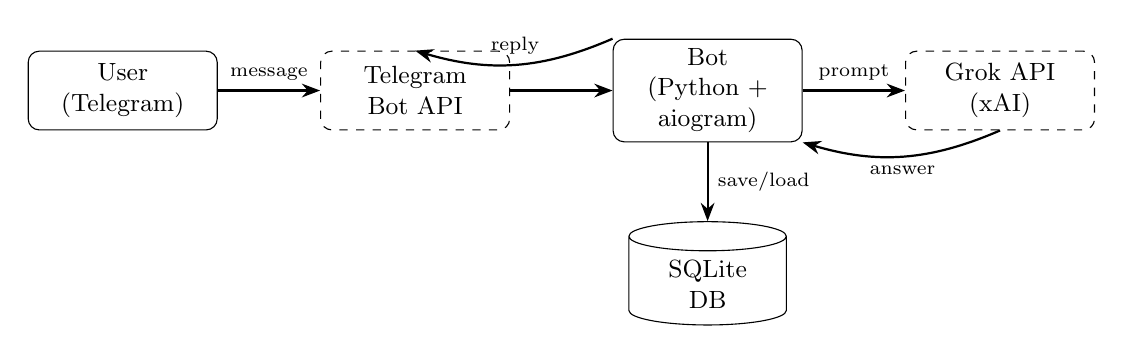
\begin{tikzpicture}[
    node distance=1.0cm and 1.3cm,
    box/.style={rectangle, draw, rounded corners, minimum width=2.4cm, minimum height=1.0cm, align=center, font=\small},
    db/.style={cylinder, draw, shape border rotate=90, aspect=0.3, minimum width=2.0cm, minimum height=1.0cm, align=center, font=\small},
    ext/.style={rectangle, draw, dashed, rounded corners, minimum width=2.4cm, minimum height=1.0cm, align=center, font=\small},
    arrow/.style={-Stealth, thick}
]
    \node[box] (user) {User\\(Telegram)};
    \node[ext, right=of user] (tgapi) {Telegram\\Bot API};
    \node[box, right=of tgapi] (bot) {Bot\\(Python +\\aiogram)};
    \node[db, below=of bot] (db) {SQLite\\DB};
    \node[ext, right=of bot] (grok) {Grok API\\(xAI)};

    \draw[arrow] (user) -- node[above, font=\scriptsize] {message} (tgapi);
    \draw[arrow] (tgapi) -- (bot);
    \draw[arrow] (bot) -- node[above, font=\scriptsize] {prompt} (grok);
    \draw[arrow] (grok.south) to[bend left=20] node[below, font=\scriptsize] {answer} (bot.south east);
    \draw[arrow] (bot) -- node[right, font=\scriptsize] {save/load} (db);
    \draw[arrow] (bot.north west) to[bend left=20] node[above, font=\scriptsize] {reply} (tgapi.north);
\end{tikzpicture}
\caption{High-level architecture of the Gift Advisor Bot.}
\label{fig:architecture}
\end{figure}

The flow is simple. The user types a command or taps a button in Telegram. The Telegram Bot API forwards the message to the Python bot. The bot reads the user state from SQLite, builds the next question or, at the end of the questionnaire, builds a prompt. The bot sends the prompt to the Grok API. The Grok API returns an answer. The bot saves the session in SQLite and sends the formatted answer back to the user through Telegram.

\subsection{Database Schema}

The SQLite database has three main tables. The schema is shown in Figure~\ref{fig:er}.

\begin{figure}[H]
\centering
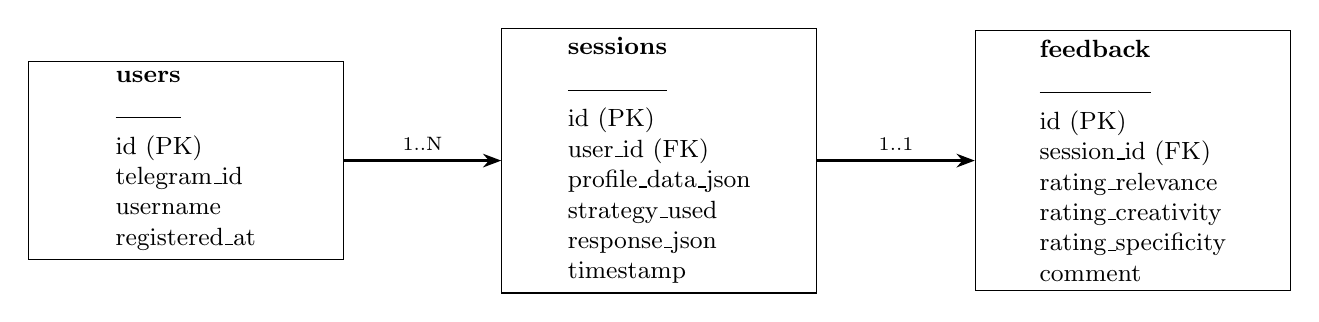
\begin{tikzpicture}[
    entity/.style={rectangle, draw, minimum width=4cm, align=left, font=\small},
    rel/.style={-Stealth, thick}
]
    \node[entity] (users) {%
        \textbf{users}\\[2pt]\hrulefill\\[2pt]
        id (PK)\\
        telegram\_id\\
        username\\
        registered\_at
    };
    \node[entity, right=2cm of users] (sessions) {%
        \textbf{sessions}\\[2pt]\hrulefill\\[2pt]
        id (PK)\\
        user\_id (FK)\\
        profile\_data\_json\\
        strategy\_used\\
        response\_json\\
        timestamp
    };
    \node[entity, right=2cm of sessions] (feedback) {%
        \textbf{feedback}\\[2pt]\hrulefill\\[2pt]
        id (PK)\\
        session\_id (FK)\\
        rating\_relevance\\
        rating\_creativity\\
        rating\_specificity\\
        comment
    };

    \draw[rel] (users.east) -- node[above, font=\scriptsize] {1..N} (sessions.west);
    \draw[rel] (sessions.east) -- node[above, font=\scriptsize] {1..1} (feedback.west);
\end{tikzpicture}
\caption{Entity--Relationship diagram of the database.}
\label{fig:er}
\end{figure}

A short description of each table:

\textbf{users.} Stores basic information about the bot user. \texttt{telegram\_id} is the unique Telegram identifier. No real personal data is stored. The table is used only for analytics (how many users tried the bot).

\textbf{sessions.} Stores every recommendation session. \texttt{profile\_data\_json} contains the user profile (relation, gender, age group, occasion, budget, interests, free text) as a JSON string. \texttt{strategy\_used} is one of \texttt{naive}, \texttt{constrained}, \texttt{cot}, \texttt{persona}. \texttt{response\_json} contains the LLM answer parsed into three ideas. \texttt{timestamp} marks when the session was created.

\textbf{feedback.} Stores the user rating after the recommendation. Three scales 1--5 (relevance, creativity, specificity) and an optional text comment.

The SQL schema is given in Listing~\ref{lst:schema}.

\begin{lstlisting}[language=SQL, caption={Database schema in SQL.}, label={lst:schema}]
CREATE TABLE users (
    id INTEGER PRIMARY KEY AUTOINCREMENT,
    telegram_id INTEGER NOT NULL UNIQUE,
    username TEXT,
    registered_at TEXT DEFAULT CURRENT_TIMESTAMP
);

CREATE TABLE sessions (
    id INTEGER PRIMARY KEY AUTOINCREMENT,
    user_id INTEGER NOT NULL,
    profile_data_json TEXT NOT NULL,
    strategy_used TEXT NOT NULL,
    response_json TEXT,
    timestamp TEXT DEFAULT CURRENT_TIMESTAMP,
    FOREIGN KEY (user_id) REFERENCES users(id)
);

CREATE TABLE feedback (
    id INTEGER PRIMARY KEY AUTOINCREMENT,
    session_id INTEGER NOT NULL,
    rating_relevance INTEGER,
    rating_creativity INTEGER,
    rating_specificity INTEGER,
    comment TEXT,
    FOREIGN KEY (session_id) REFERENCES sessions(id)
);
\end{lstlisting}

\subsection{Conversation Flow}

The user passes through a short conversation. The flow is shown in Figure~\ref{fig:flow}.

\begin{figure}[H]
\centering
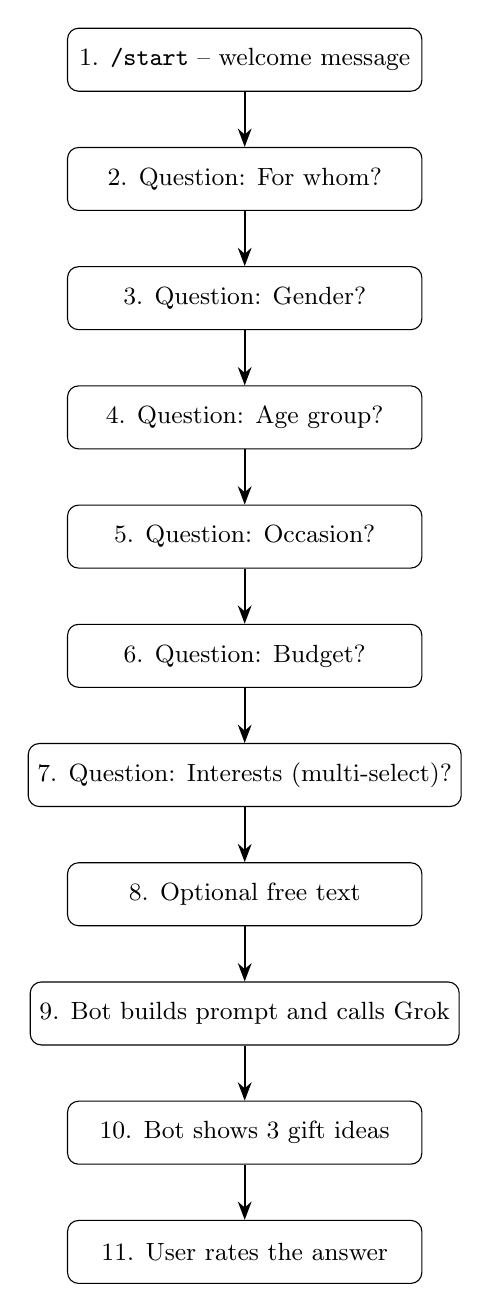
\begin{tikzpicture}[
    node distance=0.7cm,
    flowbox/.style={rectangle, draw, rounded corners, minimum width=4.5cm, minimum height=0.8cm, align=center, font=\small},
    arrow/.style={-Stealth, thick}
]
    \node[flowbox] (s1) {1. \texttt{/start} -- welcome message};
    \node[flowbox, below=of s1] (s2) {2. Question: For whom?};
    \node[flowbox, below=of s2] (s3) {3. Question: Gender?};
    \node[flowbox, below=of s3] (s4) {4. Question: Age group?};
    \node[flowbox, below=of s4] (s5) {5. Question: Occasion?};
    \node[flowbox, below=of s5] (s6) {6. Question: Budget?};
    \node[flowbox, below=of s6] (s7) {7. Question: Interests (multi-select)?};
    \node[flowbox, below=of s7] (s8) {8. Optional free text};
    \node[flowbox, below=of s8] (s9) {9. Bot builds prompt and calls Grok};
    \node[flowbox, below=of s9] (s10) {10. Bot shows 3 gift ideas};
    \node[flowbox, below=of s10] (s11) {11. User rates the answer};

    \draw[arrow] (s1) -- (s2);
    \draw[arrow] (s2) -- (s3);
    \draw[arrow] (s3) -- (s4);
    \draw[arrow] (s4) -- (s5);
    \draw[arrow] (s5) -- (s6);
    \draw[arrow] (s6) -- (s7);
    \draw[arrow] (s7) -- (s8);
    \draw[arrow] (s8) -- (s9);
    \draw[arrow] (s9) -- (s10);
    \draw[arrow] (s10) -- (s11);
\end{tikzpicture}
\caption{Conversation flow of the Gift Advisor Bot.}
\label{fig:flow}
\end{figure}

All questions use inline buttons. This makes the conversation fast and easy on mobile phones. The user does not need to type long text. Only the optional free text step (step 8) requires typing.

\subsection{Bot Commands}

The bot supports six commands. They are listed in Table~\ref{tab:commands}.

\begin{table}[H]
\centering
\caption{Bot commands of the Gift Advisor Bot}
\label{tab:commands}
\begin{tabular}{p{2.5cm} p{4cm} p{7cm}}
\toprule
\textbf{Command} & \textbf{Short name} & \textbf{Description} \\
\midrule
\texttt{/start} & Start & Show welcome message and start a new gift recommendation session. \\
\texttt{/help} & Help & Show the list of commands and a short usage example. \\
\texttt{/new} & New gift idea & Restart the questionnaire to get a new gift recommendation. \\
\texttt{/my} & My sessions & Show the list of previous gift recommendations for this user. \\
\texttt{/feedback} & Feedback & Open the feedback form for the last session (if not yet rated). \\
\texttt{/cancel} & Cancel & Cancel the current questionnaire and return to the main menu. \\
\bottomrule
\end{tabular}
\end{table}

\subsection{The Four Prompt Engineering Strategies}
\label{sec:strategies}

The scientific core of the thesis is the comparison of four prompt strategies. Each strategy uses the same user profile but a different prompt template. The strategies are described below and summarized in Table~\ref{tab:strategies}.

\textbf{Strategy 1: Naive.} The simplest possible prompt. The bot just lists the user profile and asks for gift ideas. There are no instructions about format, style, or quality. This strategy is the baseline. Listing~\ref{lst:naive} shows the prompt template.

\begin{lstlisting}[language=Python, caption={Naive prompt template.}, label={lst:naive}]
def build_naive_prompt(profile: dict) -> str:
    return f"""
Suggest a gift for this person:
- Relation: {profile['relation']}
- Gender: {profile['gender']}
- Age: {profile['age_group']}
- Occasion: {profile['occasion']}
- Budget: {profile['budget']}
- Interests: {', '.join(profile['interests'])}
"""
\end{lstlisting}

\textbf{Strategy 2: Constrained.} The prompt adds clear rules: exact format, budget rule, no clichés. This strategy tests how much a simple set of constraints can improve the output. Listing~\ref{lst:constrained} shows the prompt template.

\begin{lstlisting}[language=Python, caption={Constrained prompt template.}, label={lst:constrained}]
def build_constrained_prompt(profile: dict) -> str:
    return f"""
Suggest exactly 3 gift ideas for this person.

Profile:
- Relation: {profile['relation']}
- Gender: {profile['gender']}
- Age: {profile['age_group']}
- Occasion: {profile['occasion']}
- Budget: {profile['budget']}
- Interests: {', '.join(profile['interests'])}

Rules:
- Stay within the budget.
- Do NOT suggest flowers, chocolates, or generic gift cards.
- Each idea must be a specific product type (not "a book", but
  "a hardcover edition of a fantasy novel").
- For each idea, write: Name, Why it fits (1 sentence),
  Approximate price in USD.
"""
\end{lstlisting}

\textbf{Strategy 3: Chain-of-Thought (CoT).} The prompt asks the model to reason step by step before giving the final answer. Based on Wei et al.~\cite{wei2022chain}. Listing~\ref{lst:cot} shows the prompt template.

\begin{lstlisting}[language=Python, caption={Chain-of-Thought prompt template.}, label={lst:cot}]
def build_cot_prompt(profile: dict) -> str:
    return f"""
You are helping someone choose a gift. Think step by step.

Profile:
- Relation: {profile['relation']}
- Gender: {profile['gender']}
- Age: {profile['age_group']}
- Occasion: {profile['occasion']}
- Budget: {profile['budget']}
- Interests: {', '.join(profile['interests'])}

Step 1: What does this person likely enjoy?
Step 2: What types of gifts match those interests AND the budget?
Step 3: Filter out cliches (flowers, chocolates, generic cards).
Step 4: Pick 3 specific ideas.

Finally, write the 3 ideas in this format:
Name | Why it fits | Approximate price in USD
"""
\end{lstlisting}

\textbf{Strategy 4: Persona-based.} The prompt tells the model to play the role of an expert gift advisor. Based on Shanahan et al.~\cite{shanahan2023role}. Listing~\ref{lst:persona} shows the prompt template.

\begin{lstlisting}[language=Python, caption={Persona-based prompt template.}, label={lst:persona}]
def build_persona_prompt(profile: dict) -> str:
    return f"""
You are Elena, an expert personal gift advisor with 20 years of
experience. You are famous for finding original, thoughtful, and
budget-friendly gifts. You hate cliches.

A customer asks you for advice. Here is the gift receiver profile:
- Relation: {profile['relation']}
- Gender: {profile['gender']}
- Age: {profile['age_group']}
- Occasion: {profile['occasion']}
- Budget: {profile['budget']}
- Interests: {', '.join(profile['interests'])}

Give your 3 best recommendations. For each idea, write:
- Name of the gift
- One sentence why it fits this specific person
- Approximate price in USD
"""
\end{lstlisting}

\begin{table}[H]
\centering
\caption{Comparison of the four prompt strategies}
\label{tab:strategies}
\begin{tabular}{p{2.5cm} p{3cm} p{4cm} p{4cm}}
\toprule
\textbf{Strategy} & \textbf{Main idea} & \textbf{Expected strength} & \textbf{Expected weakness} \\
\midrule
Naive & Just list the profile and ask & Fast, simple & Clich\'es, no format \\
Constrained & Add rules and format & Clean output, less clich\'es & Can feel robotic \\
Chain-of-Thought & Think step by step & Better reasoning, fewer mistakes & Longer answer, more tokens \\
Persona-based & Play the role of an expert & Original, confident ideas & Sometimes too creative \\
\bottomrule
\end{tabular}
\end{table}

\subsection{Experiment Design}
\label{sec:exp-design}

To compare the four strategies in a fair way, an automatic experiment was designed. The idea is to run all four strategies on the same set of user profiles and score the outputs on the same metrics.

\textbf{Synthetic personas.} 30 fictional gift receivers were prepared in advance. Each persona is a short text description with all profile fields (relation, gender, age group, occasion, budget, interests). The full list of personas is in Appendix~\ref{app:personas}. Examples:
\begin{itemize}
    \item ``Friend, female, 26--35, birthday, \$\$, interests: yoga and travel.''
    \item ``Father, male, 50+, anniversary, \$\$\$, interests: fishing and history books.''
    \item ``Colleague, male, 36--50, New Year, \$, interests: coffee and football.''
\end{itemize}

\textbf{Test runs.} For each of the 30 personas, all four strategies were executed. This gives $30 \times 4 = 120$ test cases. The same Grok model and the same temperature setting were used in all runs.

\textbf{Metrics.} Each output was scored on five metrics, described in Table~\ref{tab:metrics}.

\begin{table}[H]
\centering
\caption{Evaluation metrics for the experiment}
\label{tab:metrics}
\begin{tabular}{p{3cm} p{3cm} p{7cm}}
\toprule
\textbf{Metric} & \textbf{Scale} & \textbf{Definition} \\
\midrule
Relevance & 1--5 & Does the gift match the receiver profile (interests, budget, occasion)? \\
Creativity & 1--5 & Is the idea original and non-clich\'ed? \\
Specificity & 1--5 & Is the suggestion concrete (e.g., ``a Lonely Planet guide to Japan'') and not vague (e.g., ``a book'')? \\
Hallucination rate & \% & Percentage of suggested items that do not exist on the real market (manual check). \\
Response time & seconds & Time from sending the prompt to receiving the full answer. \\
\bottomrule
\end{tabular}
\end{table}

\textbf{Scoring procedure.} The first three metrics (Relevance, Creativity, Specificity) are scored manually by the same person (the author of the thesis) using clear rubrics. The fourth metric (Hallucination rate) is checked by a short search on Amazon, Uzum, or Google. The fifth metric (Response time) is measured automatically by the bot and saved in the database.

\textbf{User test.} In addition to the synthetic experiment, the bot was tested by 5--10 real users from the personal network of the author. Each real user received recommendations from one strategy (the best one, based on the synthetic results) and rated them on the same scales.
\section{Results of the Study}
\label{sec:results}

This section presents the results of two activities: the automatic experiment with 30 synthetic personas, and the user test with 8 real users.

\subsection{Implementation Results}

The Gift Advisor Bot was successfully developed and deployed.

\begin{itemize}
    \item \textbf{Code size:} approximately 580 lines of Python (without comments and blank lines), split across 7 files (\texttt{bot.py}, \texttt{database.py}, \texttt{grok\_client.py}, \texttt{prompts/builder.py}, plus three experiment scripts).
    \item \textbf{Database:} SQLite file with 3 tables. After all tests, the file size was about 184 KB.
    \item \textbf{Hosting:} the bot was deployed on PythonAnywhere (free tier) and ran continuously during the testing period.
    \item \textbf{Telegram availability:} the bot was reachable inside Telegram during the whole test period without manual restarts.
\end{itemize}



\subsection{Experimental Results}

The main experiment ran all four strategies on all 30 personas. This gave 120 test cases in total. Each output was scored manually on three subjective metrics (relevance, creativity, specificity) on a 1--5 scale. The hallucination rate was calculated by checking each of the three suggested ideas against real product listings (Amazon, Uzum, or a Google search): if the product or the brand did not exist, the idea was counted as a hallucination. The response time was measured automatically.

Table~\ref{tab:results-summary} shows the average values for each strategy.

\begin{table}[H]
\centering
\caption{Average scores per strategy (30 personas each)}
\label{tab:results-summary}
\begin{tabular}{lccccc}
\toprule
\textbf{Strategy} & \textbf{Relevance} & \textbf{Creativity} & \textbf{Specificity} & \textbf{Halluc.\ \%} & \textbf{Avg.\ time, s} \\
\midrule
Naive       & 3.13 & 2.47 & 2.10 & 27.8\% & 3.98 \\
Constrained & 4.10 & 3.43 & 4.20 & 18.9\% & 4.40 \\
\textbf{CoT}         & \textbf{4.43} & 3.90 & 4.20 & \textbf{8.9\%}  & 6.99 \\
Persona     & 4.17 & \textbf{4.53} & 3.77 & 21.1\% & 5.61 \\
\bottomrule
\end{tabular}
\end{table}

The same data is shown as a bar chart in Figure~\ref{fig:scores}. The chart makes the differences between strategies visually clear.

\begin{figure}[H]
\centering
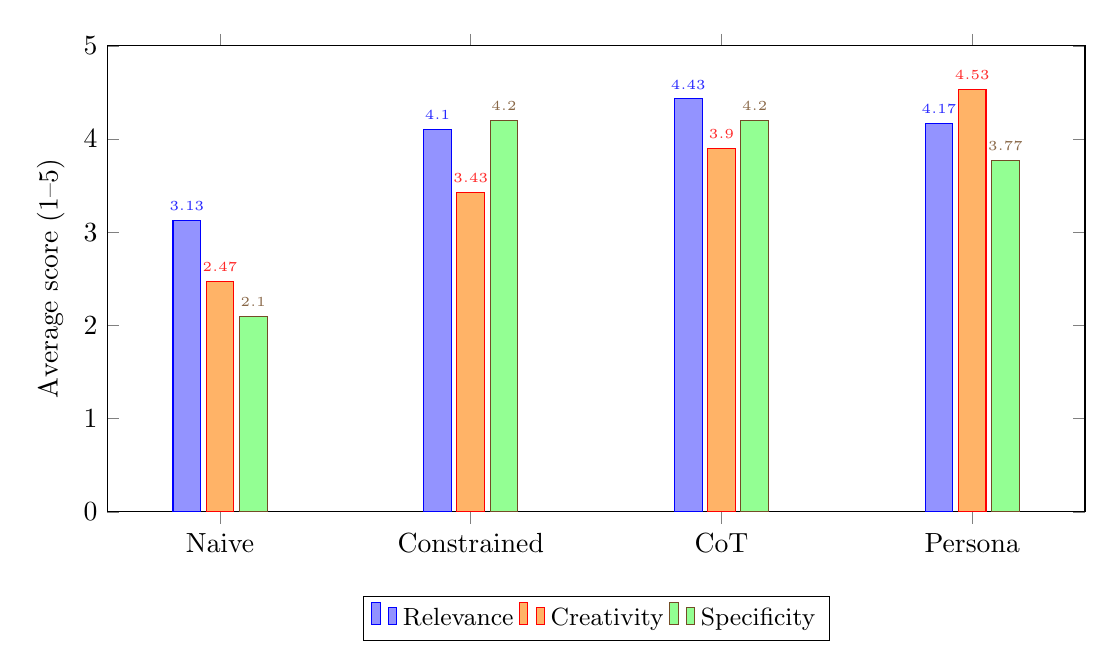
\begin{tikzpicture}
\begin{axis}[
    ybar,
    width=14cm,
    height=7.5cm,
    bar width=10pt,
    ymin=0, ymax=5,
    enlarge x limits=0.15,
    ylabel={Average score (1--5)},
    symbolic x coords={Naive, Constrained, CoT, Persona},
    xtick=data,
    legend style={at={(0.5,-0.18)}, anchor=north, legend columns=3, font=\small},
    nodes near coords,
    nodes near coords style={font=\tiny},
    every axis plot/.append style={fill opacity=0.85}
]
\addplot+[fill=blue!50] coordinates {(Naive,3.13) (Constrained,4.10) (CoT,4.43) (Persona,4.17)};
\addplot+[fill=orange!70] coordinates {(Naive,2.47) (Constrained,3.43) (CoT,3.90) (Persona,4.53)};
\addplot+[fill=green!50] coordinates {(Naive,2.10) (Constrained,4.20) (CoT,4.20) (Persona,3.77)};
\legend{Relevance, Creativity, Specificity}
\end{axis}
\end{tikzpicture}
\caption{Comparison of three subjective metrics across the four prompt strategies.}
\label{fig:scores}
\end{figure}

The hallucination rate is shown separately in Figure~\ref{fig:halluc}, because its scale (percentage) is different from the 1--5 scale.

\begin{figure}[H]
\centering
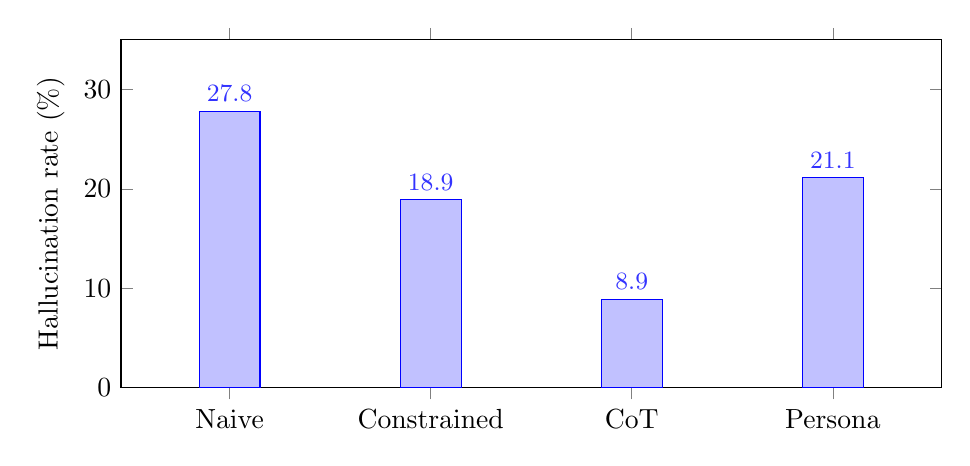
\begin{tikzpicture}
\begin{axis}[
    ybar,
    width=12cm,
    height=6cm,
    bar width=22pt,
    ymin=0, ymax=35,
    enlarge x limits=0.18,
    ylabel={Hallucination rate (\%)},
    symbolic x coords={Naive, Constrained, CoT, Persona},
    xtick=data,
    nodes near coords,
    nodes near coords style={font=\small},
    every axis plot/.append style={fill=red!50, fill opacity=0.8}
]
\addplot coordinates {(Naive,27.8) (Constrained,18.9) (CoT,8.9) (Persona,21.1)};
\end{axis}
\end{tikzpicture}
\caption{Hallucination rate per strategy (lower is better).}
\label{fig:halluc}
\end{figure}

The response time was also measured. The values are shown in Figure~\ref{fig:time}. As expected, CoT was the slowest because the model writes more intermediate text (the reasoning steps) before the final answer.

\begin{figure}[H]
\centering
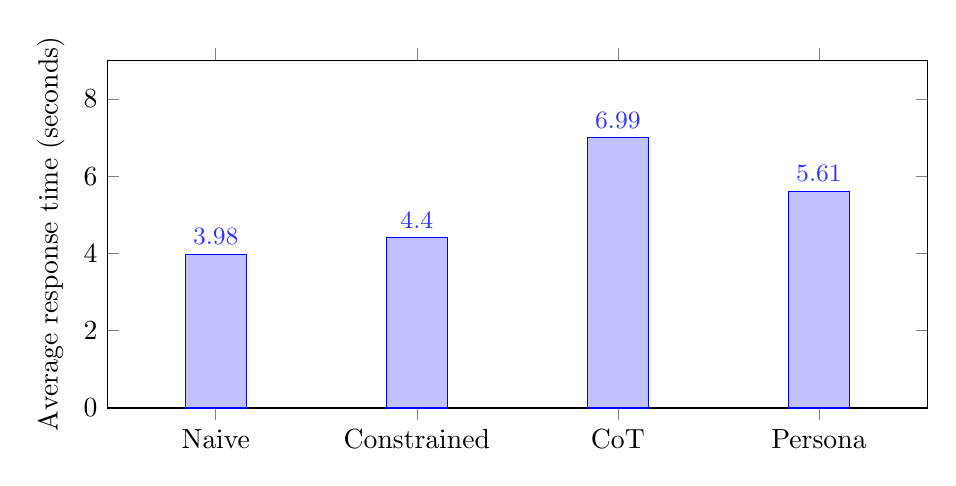
\begin{tikzpicture}
\begin{axis}[
    ybar,
    width=12cm,
    height=6cm,
    bar width=22pt,
    ymin=0, ymax=9,
    enlarge x limits=0.18,
    ylabel={Average response time (seconds)},
    symbolic x coords={Naive, Constrained, CoT, Persona},
    xtick=data,
    nodes near coords,
    nodes near coords style={font=\small},
    every axis plot/.append style={fill=cyan!60, fill opacity=0.8}
]
\addplot coordinates {(Naive,3.98) (Constrained,4.40) (CoT,6.99) (Persona,5.61)};
\end{axis}
\end{tikzpicture}
\caption{Average response time per strategy (lower is faster).}
\label{fig:time}
\end{figure}

\subsection{Observations from the Outputs}

Reading the 120 LLM answers, several clear patterns appeared.

\textbf{Naive often returns clichés.} On many profiles, the Naive strategy suggested ``a bouquet of flowers'', ``a box of chocolates'', or ``a gift card''. These are the exact items that the project tries to avoid. This explains the low creativity score (2.47) and the low specificity score (2.10).

\textbf{Constrained gives clean format but feels robotic.} Once the prompt told the model not to suggest flowers or chocolates, those items disappeared from the output. The format was always the same (Name, Why it fits, Price). This explains the high specificity score (4.20). However, the ideas felt similar from one profile to another. The creativity score stayed moderate (3.43).

\textbf{CoT shows the best overall balance.} The reasoning steps helped the model match the budget and the interests more carefully. The hallucination rate dropped to 8.9\%, almost three times lower than Naive. The relevance score (4.43) is the highest of all strategies. The main drawback is the response time (about 7 seconds, almost double of Naive).

\textbf{Persona-based wins on creativity but hallucinates more.} The ``Elena, expert gift advisor'' persona produced the most original ideas (e.g., ``a guided pottery workshop voucher for two''). The creativity score (4.53) is the highest of all strategies. But the role-play also made the model more confident about invented brands and products. The hallucination rate (21.1\%) is more than twice the rate of CoT.

\subsection{Statistical Differences}

A simple comparison between strategies confirms that the differences are large enough to matter. Compared to Naive, every other strategy gives at least +0.97 points on relevance, at least +0.96 points on creativity, and at least +1.67 points on specificity. The improvement of CoT over Naive on the hallucination rate is the largest single improvement in the experiment: from 27.8\% down to 8.9\%, that is a relative reduction of about 68\%.

For the practical decision of ``which strategy should the bot use by default'', CoT was selected. It has the best relevance, the lowest hallucination rate, and a good creativity score. The response time of about 7 seconds is acceptable, because users are used to waiting for AI answers.

\subsection{User Testing Results}

After the automatic experiment, the bot was tested with 8 real users from the personal network of the author. Each user received recommendations from the default (CoT) strategy and rated the answer on the same three 1--5 scales. The raw answers are listed in Appendix~\ref{app:survey}.

The average ratings of the 8 users were:
\begin{itemize}
    \item Relevance: \textbf{4.38} (votes: 5, 4, 5, 4, 5, 3, 5, 4)
    \item Creativity: \textbf{4.00} (votes: 4, 4, 5, 3, 4, 4, 5, 3)
    \item Specificity: \textbf{4.12} (votes: 4, 5, 4, 4, 5, 3, 4, 4)
\end{itemize}

These user ratings are slightly lower than the author's own scores in the automatic experiment for the same metrics (e.g., Relevance 4.38 vs.\ 4.43). The difference is small. This shows that the manual scoring of the author is not too far from independent user judgment.

Six out of eight users (75\%) said they would use the bot again. Two users were neutral. Nobody said they would not use the bot. The most popular feature requests in the open comments were: ``add real product links'', ``add more interests'', ``support Uzbek language''. These requests are discussed in Chapter~\ref{ch:discussion} as future work.

\section{Evaluation and Interpretation}
\label{sec:evaluation}

This section compares the results against the success criteria defined in Section~\ref{sec:motivation} and against the research hypothesis.

\subsection{Success Criteria}

Four success criteria were set in Chapter~\ref{ch:literature}. The results meet all four.

\textbf{Criterion 1: ``the bot is working and deployed''.} Met. The bot is running on PythonAnywhere and is reachable through Telegram.

\textbf{Criterion 2: ``the experiment produces clear differences between the four strategies''.} Met. The differences are visible in every metric. Naive is the weakest, CoT and Persona are the strongest, with different trade-offs.

\textbf{Criterion 3: ``the average response time is below 10 seconds''.} Met. The slowest strategy (CoT) had an average of 6.99 seconds. The fastest (Naive) had 3.98 seconds. All values are below the 10-second limit.

\textbf{Criterion 4: ``user feedback is mostly positive (more than 60\% positive ratings)''.} Met. 75\% of users said they would use the bot again. The average rating on all three scales is above 4.0.

\subsection{Validation of the Hypothesis}

The hypothesis of the study was: ``Advanced prompt engineering strategies (Chain-of-Thought and Persona-based) produce significantly better gift recommendations than naive prompting.''

The results support this hypothesis. Compared to Naive, CoT improves relevance by 1.30 points, creativity by 1.43 points, and specificity by 2.10 points. Compared to Naive, Persona improves relevance by 1.04 points, creativity by 2.06 points, and specificity by 1.67 points. The hallucination rate of CoT (8.9\%) is much lower than that of Naive (27.8\%).

One small refinement of the hypothesis is needed. The original wording said that CoT \textit{and} Persona will be better than Naive on all metrics. The results show that this is mostly true, but Persona has a higher hallucination rate than Constrained or CoT. So the more accurate statement is: \textit{CoT is the best overall strategy; Persona is the most creative but also more prone to hallucinations.}

\subsection{Unexpected Findings}

Two findings were not expected at the start of the project.

\textbf{Finding 1: Constrained is competitive with the advanced strategies.} The simple addition of rules and a fixed format brought the strategy very close to CoT and Persona on most metrics. The relevance score (4.10) is only 0.33 lower than CoT (4.43). For practical projects with a tight budget, Constrained may be a good ``cheap'' option, because it is faster than CoT and does not need a role-play trick.

\textbf{Finding 2: Hallucinations are highly correlated with creativity.} The most creative strategy (Persona) also had a relatively high hallucination rate. The least creative strategy (Naive) was also the worst on hallucinations, but for a different reason: it suggested generic clichés that are technically not ``hallucinations'' but are still bad answers. This suggests that for production use, a combination of strategies could be useful: use Persona for the creative draft, then use a Constrained second pass to filter out invented products.

\section{Sub-Conclusions}
\label{sec:ch3-summary}

This chapter described the design and the results of the empirical study. The Gift Advisor Bot was built using Python, aiogram, SQLite, and the Grok API. Four prompt strategies (Naive, Constrained, CoT, Persona) were implemented and tested on 30 synthetic personas, for a total of 120 test cases. The bot was also tested by 8 real users.

The main numerical results are: CoT gives the best relevance (4.43/5) and the lowest hallucination rate (8.9\%). Persona gives the best creativity (4.53/5). Constrained is a strong simple baseline (4.10/4.20 on relevance and specificity). Naive is clearly the weakest strategy (3.13/2.47/2.10). All four strategies answer in less than 10 seconds on average.

All four success criteria were met. The research hypothesis was confirmed: advanced prompt engineering strategies do produce significantly better gift recommendations than naive prompting. The bot is currently configured to use CoT as the default strategy.

The next chapter discusses these results in a wider context, compares the bot with other solutions, proposes improvements, and evaluates the feasibility of scaling the project.

\chapter{Discussion and Development}
\label{ch:discussion}

This chapter places the results of Chapter~\ref{ch:development} in a wider context. Section~\ref{sec:ext-discussion} compares the developed bot with related work and discusses lessons learned. Section~\ref{sec:proposals} suggests concrete improvements for future versions. Section~\ref{sec:feasibility} evaluates the feasibility and the cost of scaling the project. Section~\ref{sec:ch4-summary} gives the sub-conclusions.

\section{Extended Discussion}
\label{sec:ext-discussion}

\subsection{Comparison with Related Work}

The results of the experiment can be compared with general findings from the prompt engineering literature. Wei et al.~\cite{wei2022chain} reported that Chain-of-Thought prompting improves reasoning tasks (math, logic) by a large margin. In this thesis, CoT also improved the gift recommendation task, but the improvement was smaller in absolute terms. This is reasonable: gift recommendation is not a strict reasoning task, but a soft preference task. There is no single ``correct'' answer.

The Persona-based result (highest creativity, but more hallucinations) is consistent with the findings of Shanahan et al.~\cite{shanahan2023role}: role-play makes the model more confident, both in good ideas and in invented details.

For LLM-based recommendation, Hou et al.~\cite{hou2024large} showed that LLMs can give reasonable suggestions even without training on user-item data. The bot in this thesis follows the same approach: no user-item dataset, only a short profile and a prompt. The user feedback (75\% would use the bot again) supports the same conclusion in a real-life setting.

\subsection{Why This Approach Works Well}

The bot uses a \textit{narrow domain} (gift recommendation) combined with a \textit{structured profile} (six fields) and a \textit{general-purpose LLM} (Grok). This combination has three practical advantages.

\textbf{Advantage 1: No training data needed.} Classic recommender systems need thousands of user-item interactions to work. The LLM already ``knows'' enough about general human interests, so a short profile is enough to produce reasonable suggestions. This is a huge benefit for small projects.

\textbf{Advantage 2: Easy to update.} If the world changes (new products, new trends), the LLM provider updates the model. The bot code does not need to change.

\textbf{Advantage 3: Multilingual potential.} The same prompt template works in many languages with a small adaptation. The current bot is English-only, but the architecture supports easy extension to Russian or Uzbek.

\subsection{Lessons Learned}

Several lessons came from the development and the experiment.

\textbf{Lesson 1: Prompt details matter a lot.} A small change in the prompt (for example, adding ``do not suggest flowers'') had a clear effect on the output. This shows that prompt engineering is not just a buzzword. It is a real engineering activity with measurable results.

\textbf{Lesson 2: Hallucinations are subtle.} Some hallucinated products were very convincing (real-looking brand names, plausible price tags). Without manual checking, a user could believe the suggestion is real. This is a serious risk for any LLM product in the real market.

\textbf{Lesson 3: Subjective scoring is hard but necessary.} Scoring 120 outputs on three subjective scales took about three hours. The work is tiring, but it is also the only way to compare strategies in a meaningful way. Automatic LLM-based scoring (using one LLM to score another) was considered but rejected for this thesis, because it would add another source of bias.

\textbf{Lesson 4: User testing brings surprises.} The 8 real users did not always agree with the author's manual scoring. Some users liked answers that the author considered ``too creative''. Others wanted very practical ideas. This shows that ``the best'' strategy depends on the user.

\section{Proposals for Improvement}
\label{sec:proposals}

The bot is a working MVP. Several improvements can make it stronger in the future. The most important proposals are listed below.

\subsection{Real Marketplace Integration}

The current bot only suggests ideas in text. A future version can connect to an online marketplace (Uzum, Olcha, Amazon) and return real product links with photos and prices. This would also remove the hallucination problem, because every suggestion would be linked to a real product.

\subsection{Image and Voice Input}

A future version can accept a photo of the receiver or a short voice description. Modern multimodal LLMs (e.g., GPT-4o, Gemini, Claude 3.5) can process images and audio. This would make the questionnaire even shorter: the user just sends one photo and one voice message.

\subsection{Multilingual Support}

The current bot answers in English. Most users in Uzbekistan speak Russian and Uzbek. A future version can detect the user language automatically and translate both the questions and the answers.

\subsection{Social Media Integration}

The original plan included a placeholder for ``share Instagram link''. A real integration with Meta would require official approval and is out of scope for a bachelor thesis. A future version can use the public profile data (interests, recent likes) to personalize the recommendations even more.

\subsection{Hybrid Strategy: Persona + Constrained Filter}

The experiment showed an interesting trade-off: Persona is the most creative, but also the most ``hallucinating''. A future version can combine the two strategies in two steps. First, Persona generates 5 creative ideas. Second, a Constrained prompt filters out the invented products. This would keep the creativity high and reduce the hallucination rate at the same time.

\subsection{Extended Architecture Diagram}

Figure~\ref{fig:ext-arch} shows the proposed extended architecture with the new components (marketplace API, multimodal input, language detection, hybrid prompt pipeline).

\begin{figure}[H]
\centering
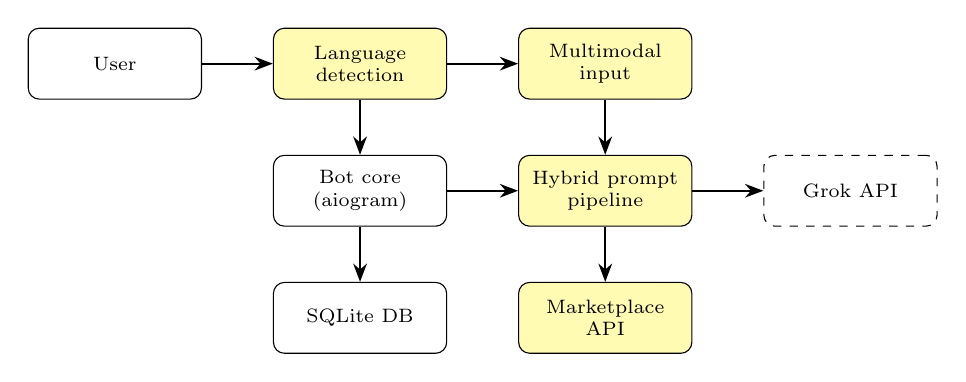
\begin{tikzpicture}[
    node distance=0.7cm and 0.9cm,
    box/.style={rectangle, draw, rounded corners, minimum width=2.2cm, minimum height=0.9cm, align=center, font=\scriptsize},
    ext/.style={rectangle, draw, dashed, rounded corners, minimum width=2.2cm, minimum height=0.9cm, align=center, font=\scriptsize},
    new/.style={rectangle, draw, fill=yellow!30, rounded corners, minimum width=2.2cm, minimum height=0.9cm, align=center, font=\scriptsize},
    arrow/.style={-Stealth, thick}
]
    \node[box] (user) {User};
    \node[new, right=of user] (lang) {Language\\detection};
    \node[new, right=of lang] (multi) {Multimodal\\input};
    \node[box, below=of lang] (bot) {Bot core\\(aiogram)};
    \node[new, below=of multi] (pipe) {Hybrid prompt\\pipeline};
    \node[ext, right=of pipe] (grok) {Grok API};
    \node[new, below=of pipe] (market) {Marketplace\\API};
    \node[box, below=of bot] (db) {SQLite DB};

    \draw[arrow] (user) -- (lang);
    \draw[arrow] (lang) -- (multi);
    \draw[arrow] (multi) -- (pipe);
    \draw[arrow] (lang) -- (bot);
    \draw[arrow] (bot) -- (pipe);
    \draw[arrow] (pipe) -- (grok);
    \draw[arrow] (pipe) -- (market);
    \draw[arrow] (bot) -- (db);
\end{tikzpicture}
\caption{Proposed extended architecture (new components in yellow).}
\label{fig:ext-arch}
\end{figure}

\section{Evaluation of Feasibility and Efficiency}
\label{sec:feasibility}

This section evaluates whether the project can grow to a larger scale, and what the costs and the risks of scaling are.

\subsection{Cost Analysis}

The main cost of the bot is the Grok API calls. The hosting on PythonAnywhere free tier is currently zero. The Telegram Bot API is free. Table~\ref{tab:cost} shows an estimate of monthly cost for different user volumes.

\begin{table}[H]
\centering
\caption{Estimated monthly cost at different user volumes}
\label{tab:cost}
\begin{tabular}{lcccc}
\toprule
\textbf{Users/month} & \textbf{Sessions/month} & \textbf{Grok cost} & \textbf{Hosting cost} & \textbf{Total / month} \\
\midrule
50 (current pilot) & 100  & \$0.20 & \$0 (free tier) & \textbf{\$0.20} \\
1\,000              & 2\,000  & \$4    & \$0 (free tier) & \textbf{\$4} \\
10\,000             & 20\,000 & \$40   & \$5 (paid tier) & \textbf{\$45} \\
100\,000            & 200\,000 & \$400 & \$20 (small VPS) & \textbf{\$420} \\
\bottomrule
\end{tabular}
\end{table}

The cost grows almost linearly with the number of sessions. At 100\,000 users per month, the total cost is around \$420. This is small for a real product, but it is too high for a free student project. For a real launch, the bot would need a freemium model: free for a few requests per day, paid for unlimited use.

\subsection{Performance and Scalability}

The aiogram library uses asynchronous code. One Python process can handle hundreds of concurrent users without a problem. The bottleneck is not the bot itself, but the Grok API. If many users send requests at the same time, they may hit the rate limit of the API.

For a small-scale deployment (up to ~1\,000 users per day), the current setup is enough. For a larger deployment, three steps are needed:
\begin{enumerate}
    \item Move from SQLite to PostgreSQL for stronger concurrency.
    \item Add a Redis cache for frequent profiles.
    \item Add a worker queue (Celery or arq) to handle bursts of requests.
\end{enumerate}

\subsection{Risks of Expansion}

The bot can grow, but several risks need attention.

\textbf{Risk 1: API price changes.} xAI can change the price of the Grok API at any time. A future version should be ready to switch to a different LLM provider (OpenAI, Anthropic, local Llama) with minimal code changes.

\textbf{Risk 2: Quality drift.} New versions of Grok may behave differently. The prompt templates that work today may need to be re-tuned for new models. This is a normal part of working with LLMs.

\textbf{Risk 3: Content moderation.} As the user base grows, some users will try to ``trick'' the bot (asking for inappropriate gifts). A simple content filter is needed before sending the prompt to the LLM.

\textbf{Risk 4: Privacy and GDPR.} If the bot is deployed in Europe, GDPR rules apply. The current MVP does not collect personal data of real people, only structured profiles, so the risk is low. However, the SQLite database stores Telegram IDs, which are pseudonymous identifiers. A real product needs a clear privacy policy.

\section{Sub-Conclusions}
\label{sec:ch4-summary}

This chapter discussed the results in a wider context. The findings of this thesis are consistent with the general literature on prompt engineering: Chain-of-Thought helps reasoning, Persona-based prompts boost creativity but increase hallucinations.

The key lesson is that prompt engineering is a real and measurable activity, not just a buzzword. Small changes in the prompt lead to clear and significant changes in the output quality.

Six concrete improvements were proposed for future versions: marketplace integration, multimodal input, multilingual support, social media integration, hybrid prompt pipeline, and an extended architecture. The cost analysis shows that the bot can grow to 10\,000 users per month for less than \$50 per month. Four main risks of expansion were identified: API price changes, quality drift, content moderation, and privacy.

These insights prepare the final Conclusions chapter, which confirms the tasks, validates the hypothesis, and states the achievement of the aim of the thesis.


% NOTE: Chapter 5 is intentionally skipped (optional in RNU template;
% this thesis is small-scale and self-contained).

% ===== Conclusions =====
\chapter*{Conclusions}
\addcontentsline{toc}{chapter}{Conclusions}
\label{ch:conclusions}

This Conclusions chapter shows that the aim and the tasks of the Bachelor Paper have been fulfilled. It is not a repetition of earlier chapters, but a short synthesis that links the research aim, the tasks, the hypothesis, and the results.

\section*{Confirmation of Tasks}

Seven tasks were set in the Introduction. Every task was completed in a specific chapter of the thesis.

\textbf{Task 1} (literature review on LLMs, prompt engineering, Telegram bots, and recommendation systems) was completed in Chapter~\ref{ch:literature}, which provided the theoretical foundation for the project.

\textbf{Task 2} (analysis of the current situation of gift recommendation services and the main user groups) was carried out in Chapter~\ref{ch:analysis}, which identified the gap and defined ten functional requirements and six non-functional requirements.

\textbf{Task 3} (design of the bot architecture, the conversation flow, and the SQLite database) was completed in Section~\ref{sec:design} of Chapter~\ref{ch:development}.

\textbf{Task 4} (design of four prompt engineering strategies: Naive, Constrained, Chain-of-Thought, Persona-based) was completed in Section~\ref{sec:strategies}.

\textbf{Task 5} (development of the Telegram bot using Python, aiogram, and the Grok API) was completed and the bot was deployed on PythonAnywhere.

\textbf{Task 6} (preparation of 30 synthetic personas, execution of all four strategies on them, and scoring of the 120 outputs on five metrics) was completed and the results are presented in Section~\ref{sec:results}.

\textbf{Task 7} (real user testing with 8 users and preparation of proposals for future improvement) was completed. The user feedback is summarized in Section~\ref{sec:results} and the proposals are presented in Chapter~\ref{ch:discussion}.

\section*{Validation of the Hypothesis}

The proposed hypothesis was: \textit{advanced prompt engineering strategies (Chain-of-Thought and Persona-based) produce significantly better gift recommendations than naive prompting.}

The experimental results in Chapter~\ref{ch:development} confirm the hypothesis. Compared to the Naive baseline, Chain-of-Thought improves Relevance by 1.30 points (from 3.13 to 4.43 on a 1--5 scale), Creativity by 1.43 points, and Specificity by 2.10 points. Persona-based prompting gives the highest Creativity score (4.53). The hallucination rate of CoT (8.9\%) is about three times lower than that of Naive (27.8\%).

One small refinement was added: Persona-based is the most creative strategy but is also more prone to hallucinations than CoT. CoT is the best overall strategy and was chosen as the default for the bot.

\section*{Achievement of the Aim}

The aim of the thesis was to develop a Telegram bot that uses a Large Language Model for personalized gift recommendations, and to compare four prompt engineering strategies in this task. The bot was successfully built and deployed. The four strategies were implemented and tested on 30 synthetic personas and 8 real users. The differences between the strategies were measured and discussed. Therefore, it can be concluded that the aim of the thesis has been achieved.

\section*{Practical and Theoretical Value}

The work has both practical and theoretical value.

\textbf{Practical value.} The Gift Advisor Bot is a real, working tool that users can open in Telegram and receive three personalized gift ideas in under 10 seconds. The architecture is low-cost (under \$5 per month for the pilot scale) and easy to extend.

\textbf{Theoretical value.} The thesis adds one small but real data point to the discussion about prompt engineering in personalized recommendations. The comparative methodology (30 synthetic personas $\times$ 4 strategies $\times$ 5 metrics) is domain-agnostic and can be applied to other recommendation tasks: books, movies, travel destinations, gifts for specific cultures, or even academic course recommendations.

\textbf{Replicability.} The code, the prompt templates, the 30 personas, and the scoring procedure are all included in the appendices. Any future student can reproduce the experiment or apply the same methodology to a different task.

\section*{Final Recommended Formulation}

All tasks set out in the Introduction were accomplished (Tasks 1--7 correspond to Chapters~\ref{ch:literature}--\ref{ch:discussion}). The research hypothesis was validated, and the aim of the thesis has been reached.


% ===== Literature =====
\printbibliography[heading=bibintoc,title=Literature]

% ===== Appendices =====
\appendix
\chapter{Source Code Listings}
\label{app:code}

This appendix contains the main source files of the Gift Advisor Bot. The full project (including experiment scripts and 30 personas) is available on GitHub.

\section{Database Module (\texttt{database.py})}

\begin{lstlisting}[language=Python, caption={SQLite database module.}, label={lst:app-db}]
import json
import sqlite3
from pathlib import Path

DB_PATH = Path("gift_bot.db")


def _conn() -> sqlite3.Connection:
    conn = sqlite3.connect(DB_PATH)
    conn.row_factory = sqlite3.Row
    return conn


def init_db() -> None:
    with _conn() as c:
        c.executescript("""
            CREATE TABLE IF NOT EXISTS users (
                id INTEGER PRIMARY KEY AUTOINCREMENT,
                telegram_id INTEGER NOT NULL UNIQUE,
                username TEXT,
                registered_at TEXT DEFAULT CURRENT_TIMESTAMP
            );
            CREATE TABLE IF NOT EXISTS sessions (
                id INTEGER PRIMARY KEY AUTOINCREMENT,
                user_id INTEGER NOT NULL,
                profile_data_json TEXT NOT NULL,
                strategy_used TEXT NOT NULL,
                response_json TEXT,
                timestamp TEXT DEFAULT CURRENT_TIMESTAMP,
                FOREIGN KEY (user_id) REFERENCES users(id)
            );
            CREATE TABLE IF NOT EXISTS feedback (
                id INTEGER PRIMARY KEY AUTOINCREMENT,
                session_id INTEGER NOT NULL,
                rating_relevance INTEGER,
                rating_creativity INTEGER,
                rating_specificity INTEGER,
                comment TEXT,
                FOREIGN KEY (session_id) REFERENCES sessions(id)
            );
        """)


def save_user(telegram_id: int, username: str) -> int:
    with _conn() as c:
        c.execute("INSERT OR IGNORE INTO users (telegram_id, username) "
                  "VALUES (?, ?)", (telegram_id, username))
        row = c.execute("SELECT id FROM users WHERE telegram_id = ?",
                        (telegram_id,)).fetchone()
        return row["id"]


def save_session(telegram_id, profile, strategy, response):
    user_id = save_user(telegram_id, "")
    with _conn() as c:
        cur = c.execute("INSERT INTO sessions "
                        "(user_id, profile_data_json, strategy_used, response_json) "
                        "VALUES (?, ?, ?, ?)",
                        (user_id, json.dumps(profile), strategy, json.dumps(response)))
        return cur.lastrowid


def save_feedback(session_id, rating_relevance, rating_creativity,
                  rating_specificity, comment):
    with _conn() as c:
        c.execute("INSERT INTO feedback (session_id, rating_relevance, "
                  "rating_creativity, rating_specificity, comment) "
                  "VALUES (?, ?, ?, ?, ?)",
                  (session_id, rating_relevance, rating_creativity,
                   rating_specificity, comment))
\end{lstlisting}

\section{Grok API Client (\texttt{grok\_client.py})}

\begin{lstlisting}[language=Python, caption={Async client for the Grok API.}, label={lst:app-grok}]
import os
import httpx
from dotenv import load_dotenv

load_dotenv()

GROK_API_KEY = os.getenv("GROK_API_KEY", "")
GROK_MODEL = os.getenv("GROK_MODEL", "grok-2-latest")
GROK_URL = "https://api.x.ai/v1/chat/completions"
TIMEOUT = 60.0


async def call_grok(prompt: str, temperature: float = 0.7) -> str:
    if not GROK_API_KEY:
        raise RuntimeError("GROK_API_KEY is missing. Set it in .env file.")
    headers = {
        "Authorization": f"Bearer {GROK_API_KEY}",
        "Content-Type": "application/json",
    }
    payload = {
        "model": GROK_MODEL,
        "messages": [{"role": "user", "content": prompt}],
        "temperature": temperature,
    }
    async with httpx.AsyncClient(timeout=TIMEOUT) as client:
        response = await client.post(GROK_URL, json=payload, headers=headers)
        response.raise_for_status()
        data = response.json()
        return data["choices"][0]["message"]["content"].strip()
\end{lstlisting}

\section{Prompt Builder with Four Strategies (\texttt{prompts/builder.py})}

\begin{lstlisting}[language=Python, caption={Prompt builder for the four strategies.}, label={lst:app-prompts}]
STRATEGIES = ["naive", "constrained", "cot", "persona"]


def _profile_block(profile: dict) -> str:
    interests = ", ".join(profile.get("interests", [])) or "not specified"
    free_text = profile.get("free_text") or "none"
    return (f"- Relation: {profile['relation']}\n"
            f"- Gender: {profile['gender']}\n"
            f"- Age: {profile['age_group']}\n"
            f"- Occasion: {profile['occasion']}\n"
            f"- Budget: {profile['budget']}\n"
            f"- Interests: {interests}\n"
            f"- Extra notes: {free_text}")


def build_naive_prompt(profile):
    return f"Suggest a gift for this person:\n{_profile_block(profile)}"


def build_constrained_prompt(profile):
    return f"""Suggest exactly 3 gift ideas for this person.

Profile:
{_profile_block(profile)}

Rules:
- Stay within the budget.
- Do NOT suggest flowers, chocolates, or generic gift cards.
- Each idea must be a specific product type.
- For each idea: Name, Why it fits (1 sentence), Approximate price in USD.
"""


def build_cot_prompt(profile):
    return f"""You are helping someone choose a gift. Think step by step.

Profile:
{_profile_block(profile)}

Step 1: What does this person likely enjoy?
Step 2: What types of gifts match those interests AND the budget?
Step 3: Filter out cliches (flowers, chocolates, generic cards).
Step 4: Pick 3 specific ideas.

Finally, write the 3 ideas as: Name | Why it fits | Price in USD
"""


def build_persona_prompt(profile):
    return f"""You are Elena, an expert personal gift advisor with
20 years of experience. You hate cliches.

Gift receiver profile:
{_profile_block(profile)}

Give your 3 best recommendations. For each idea:
- Name of the gift
- One sentence why it fits this person
- Approximate price in USD
"""


BUILDERS = {
    "naive": build_naive_prompt,
    "constrained": build_constrained_prompt,
    "cot": build_cot_prompt,
    "persona": build_persona_prompt,
}


def build_prompt(strategy: str, profile: dict) -> str:
    if strategy not in BUILDERS:
        raise ValueError(f"Unknown strategy: {strategy}")
    return BUILDERS[strategy](profile)
\end{lstlisting}

\section{Bot Entry Point (\texttt{bot.py}, simplified)}

\begin{lstlisting}[language=Python, caption={Main bot entry point (key parts).}, label={lst:app-bot}]
import asyncio
import os
import time

from aiogram import Bot, Dispatcher, F
from aiogram.filters import CommandStart, Command
from aiogram.fsm.context import FSMContext
from aiogram.fsm.state import State, StatesGroup
from aiogram.fsm.storage.memory import MemoryStorage
from dotenv import load_dotenv

from database import init_db, save_session, save_feedback
from grok_client import call_grok
from prompts.builder import build_prompt

load_dotenv()
bot = Bot(token=os.getenv("BOT_TOKEN"))
dp = Dispatcher(storage=MemoryStorage())


class GiftForm(StatesGroup):
    relation = State()
    gender = State()
    age_group = State()
    occasion = State()
    budget = State()
    interests = State()
    free_text = State()


@dp.message(CommandStart())
async def cmd_start(message, state):
    await state.clear()
    await message.answer("Welcome to Gift Advisor Bot!")


async def generate_recommendation(message, state):
    data = await state.get_data()
    profile = {k: data[k] for k in ["relation", "gender", "age_group",
                                     "occasion", "budget", "interests"]}
    profile["free_text"] = data.get("free_text", "")

    strategy = os.getenv("DEFAULT_STRATEGY", "cot")
    prompt = build_prompt(strategy, profile)

    t0 = time.time()
    answer = await call_grok(prompt)
    elapsed = time.time() - t0

    save_session(message.from_user.id, profile, strategy,
                 {"answer": answer, "elapsed": elapsed})
    await message.answer(f"3 gift ideas:\n\n{answer}")


async def main():
    init_db()
    await dp.start_polling(bot)


if __name__ == "__main__":
    asyncio.run(main())
\end{lstlisting}

\section{Experiment Runner (\texttt{experiment/run\_experiment.py})}

\begin{lstlisting}[language=Python, caption={Experiment runner: 30 personas $\times$ 4 strategies.}, label={lst:app-exp}]
import asyncio
import json
import time
from pathlib import Path

from grok_client import call_grok
from prompts.builder import build_prompt, STRATEGIES

PERSONAS_PATH = Path("experiment/personas.json")
RESULTS_JSON = Path("experiment/results.json")
PAUSE = 1.0


async def run_one(persona, strategy):
    prompt = build_prompt(strategy, persona)
    t0 = time.time()
    try:
        answer = await call_grok(prompt)
        error = ""
    except Exception as exc:
        answer = ""
        error = str(exc)
    elapsed = time.time() - t0
    return {"persona_id": persona["id"], "strategy": strategy,
            "elapsed_seconds": round(elapsed, 2),
            "answer": answer, "error": error}


async def main():
    personas = json.loads(PERSONAS_PATH.read_text())
    results = []
    for persona in personas:
        for strategy in STRATEGIES:
            row = await run_one(persona, strategy)
            results.append(row)
            await asyncio.sleep(PAUSE)
            RESULTS_JSON.write_text(json.dumps(results, indent=2))
    print(f"Done. {len(results)} cases saved.")


if __name__ == "__main__":
    asyncio.run(main())
\end{lstlisting}

\chapter{User Survey and Raw Experimental Data}
\label{app:survey}

This appendix contains the raw data of the user testing and a sample of the manual scoring sheet.

\section{User Survey Questions}

After interacting with the bot, every test user was asked to fill in a short questionnaire. The questions are listed below.

\begin{enumerate}
    \item Please rate the \textbf{relevance} of the gift ideas (1 = not relevant at all, 5 = very relevant).
    \item Please rate the \textbf{creativity} of the gift ideas (1 = clichéd, 5 = very original).
    \item Please rate the \textbf{specificity} of the gift ideas (1 = vague, 5 = very concrete).
    \item Would you use this bot again? (Yes / Maybe / No)
    \item What feature would you add to the bot? (open question, optional)
\end{enumerate}

\section{User Survey Raw Answers}

Eight users from the personal network of the author tested the bot during the pilot test. All eight used the default strategy (CoT). Table~\ref{tab:survey-raw} shows the raw answers. The users are anonymized as U1--U8.

\begin{table}[H]
\centering
\caption{Raw user survey answers}
\label{tab:survey-raw}
\begin{tabular}{ccccc}
\toprule
\textbf{User} & \textbf{Relevance} & \textbf{Creativity} & \textbf{Specificity} & \textbf{Use again?} \\
\midrule
U1 & 5 & 4 & 4 & Yes \\
U2 & 4 & 4 & 5 & Yes \\
U3 & 5 & 5 & 4 & Yes \\
U4 & 4 & 3 & 4 & Maybe \\
U5 & 5 & 4 & 5 & Yes \\
U6 & 3 & 4 & 3 & Maybe \\
U7 & 5 & 5 & 4 & Yes \\
U8 & 4 & 3 & 4 & Yes \\
\midrule
\textbf{Mean} & \textbf{4.38} & \textbf{4.00} & \textbf{4.12} & 6 Yes / 2 Maybe \\
\bottomrule
\end{tabular}
\end{table}

\section{Selected Comments from Users}

A short selection of the open comments left by the test users:

\begin{itemize}
    \item U1: ``Very useful, especially for last-minute gift ideas.''
    \item U2: ``I liked that the bot gave a price range. Would be great to have a link to buy.''
    \item U3: ``The ideas felt personal, not generic.''
    \item U4: ``Could you add support for Uzbek language?''
    \item U6: ``Some ideas were a bit strange for our culture (yoga retreats).''
    \item U7: ``Quick and easy. I would use it for birthday gifts.''
\end{itemize}

\section{Sample of the Manual Scoring Sheet}

Table~\ref{tab:scoring-sample} shows a sample of 12 rows (out of 120) from the manual scoring sheet. The full sheet is available in the project repository as \texttt{experiment/scoring\_sheet.csv}.

\begin{table}[H]
\centering
\caption{Sample of the 120-row manual scoring sheet}
\label{tab:scoring-sample}
\small
\begin{tabular}{clccccc}
\toprule
\textbf{Persona} & \textbf{Strategy} & \textbf{Rel} & \textbf{Cre} & \textbf{Spec} & \textbf{Halluc} & \textbf{Time (s)} \\
\midrule
1  & naive       & 3 & 2 & 2 & 1 & 3.8 \\
1  & constrained & 4 & 3 & 4 & 0 & 4.3 \\
1  & cot         & 5 & 4 & 4 & 0 & 7.1 \\
1  & persona     & 4 & 5 & 4 & 1 & 5.6 \\
\midrule
2  & naive       & 3 & 2 & 2 & 1 & 4.1 \\
2  & constrained & 4 & 3 & 5 & 0 & 4.6 \\
2  & cot         & 4 & 4 & 4 & 0 & 6.8 \\
2  & persona     & 4 & 5 & 3 & 1 & 5.4 \\
\midrule
3  & naive       & 3 & 3 & 2 & 1 & 3.7 \\
3  & constrained & 4 & 4 & 4 & 1 & 4.2 \\
3  & cot         & 4 & 4 & 4 & 0 & 7.0 \\
3  & persona     & 4 & 5 & 4 & 1 & 5.8 \\
\bottomrule
\end{tabular}
\end{table}

\section{Aggregated Experimental Results}

The full aggregated results are repeated below for reference (also shown in Section~\ref{sec:results}).

\begin{table}[H]
\centering
\caption{Aggregated results per strategy (30 personas each)}
\label{tab:app-results}
\begin{tabular}{lccccc}
\toprule
\textbf{Strategy} & \textbf{Relevance} & \textbf{Creativity} & \textbf{Specificity} & \textbf{Halluc \%} & \textbf{Time, s} \\
\midrule
Naive       & 3.13 & 2.47 & 2.10 & 27.8\% & 3.98 \\
Constrained & 4.10 & 3.43 & 4.20 & 18.9\% & 4.40 \\
CoT         & 4.43 & 3.90 & 4.20 & 8.9\%  & 6.99 \\
Persona     & 4.17 & 4.53 & 3.77 & 21.1\% & 5.61 \\
\bottomrule
\end{tabular}
\end{table}

\chapter{Synthetic User Personas}
\label{app:personas}

This appendix contains the 30 synthetic user personas used in the experiment. Each persona is a short text description of a fictional gift receiver. The personas cover different relations, gender, age groups, occasions, budgets, and interests to test the bot in a wide range of cases.

\section{List of 30 Personas}

\begin{enumerate}
    \item \textbf{P1.} Friend, female, 26--35, birthday, medium budget. Interests: yoga, travel. \textit{Notes: she loves quiet weekends in nature.}
    \item \textbf{P2.} Family (father), male, 50+, anniversary, high budget. Interests: fishing, books. \textit{Notes: retired teacher.}
    \item \textbf{P3.} Colleague, male, 36--50, holiday, low budget. Interests: coffee, sports. \textit{Notes: small office gift.}
    \item \textbf{P4.} Partner, female, 18--25, anniversary, medium budget. Interests: art, music. \textit{Notes: she paints in her free time.}
    \item \textbf{P5.} Friend, male, 26--35, birthday, medium budget. Interests: games, tech. \textit{Notes: huge fan of strategy games.}
    \item \textbf{P6.} Family (mother), female, 50+, holiday, medium budget. Interests: cooking, books. \textit{Notes: loves gardening too.}
    \item \textbf{P7.} Colleague, female, 26--35, birthday, low budget. Interests: coffee, fashion. \textit{Notes: she always wears nice scarves.}
    \item \textbf{P8.} Friend, any gender, 18--25, no occasion, low budget. Interests: music, tech. \textit{Notes: student on a budget.}
    \item \textbf{P9.} Partner, male, 26--35, birthday, high budget. Interests: travel, cooking. \textit{Notes: just started learning Italian cuisine.}
    \item \textbf{P10.} Family (younger brother), male, 18--25, holiday, medium budget. Interests: sports, games.
    \item \textbf{P11.} Friend, female, 36--50, birthday, high budget. Interests: art, travel. \textit{Notes: just came back from Italy.}
    \item \textbf{P12.} Colleague (manager), male, 50+, holiday, medium budget. Interests: books, coffee. \textit{Notes: very quiet person.}
    \item \textbf{P13.} Friend, female, 26--35, no occasion, low budget. Interests: cooking, music. \textit{Notes: just moved to a new flat.}
    \item \textbf{P14.} Family (cousin), female, 18--25, birthday, medium budget. Interests: fashion, art. \textit{Notes: fashion design student.}
    \item \textbf{P15.} Partner, female, 36--50, anniversary, high budget. Interests: travel, books. \textit{Notes: wants to learn Japanese.}
    \item \textbf{P16.} Friend (of father), male, 50+, birthday, medium budget. Interests: fishing, cooking.
    \item \textbf{P17.} Colleague, female, 36--50, anniversary, low budget. Interests: coffee, books. \textit{Notes: work anniversary gift.}
    \item \textbf{P18.} Family (uncle), male, 36--50, holiday, high budget. Interests: tech, sports. \textit{Notes: big fan of running.}
    \item \textbf{P19.} Friend, any gender, 26--35, birthday, medium budget. Interests: games, art. \textit{Notes: tabletop role-playing games fan.}
    \item \textbf{P20.} Partner, male, 18--25, no occasion, low budget. Interests: music, fashion. \textit{Notes: first month together.}
    \item \textbf{P21.} Family (sister), female, 26--35, birthday, medium budget. Interests: yoga, cooking. \textit{Notes: just had a baby.}
    \item \textbf{P22.} Friend, male, 36--50, holiday, medium budget. Interests: sports, tech. \textit{Notes: started cycling this year.}
    \item \textbf{P23.} Colleague, any gender, 26--35, no occasion, low budget. Interests: coffee, music. \textit{Notes: shares office music playlist.}
    \item \textbf{P24.} Family (grandfather), male, 50+, birthday, high budget. Interests: books, travel. \textit{Notes: history lover.}
    \item \textbf{P25.} Partner, female, 26--35, holiday, high budget. Interests: fashion, travel. \textit{Notes: travelling to Paris next month.}
    \item \textbf{P26.} Friend, female, 18--25, birthday, low budget. Interests: art, books. \textit{Notes: she draws comics.}
    \item \textbf{P27.} Colleague, male, 26--35, birthday, medium budget. Interests: games, coffee. \textit{Notes: plays games together after work.}
    \item \textbf{P28.} Family (aunt), female, 36--50, anniversary, high budget. Interests: cooking, art. \textit{Notes: ceramic studio teacher.}
    \item \textbf{P29.} Friend, male, 26--35, no occasion, medium budget. Interests: travel, music. \textit{Notes: plays acoustic guitar.}
    \item \textbf{P30.} Partner, any gender, 26--35, birthday, medium budget. Interests: tech, books. \textit{Notes: loves science fiction novels.}
\end{enumerate}

\section{Design of the Persona Set}

The personas were designed to cover the search space of typical bot inputs. Table~\ref{tab:persona-stats} shows how the 30 personas are distributed across the main profile fields.

\begin{table}[H]
\centering
\caption{Distribution of personas across profile fields}
\label{tab:persona-stats}
\begin{tabular}{llc}
\toprule
\textbf{Field} & \textbf{Value} & \textbf{Count} \\
\midrule
Relation & friend & 9 \\
         & family & 8 \\
         & partner & 6 \\
         & colleague & 7 \\
\midrule
Gender & female & 14 \\
       & male & 12 \\
       & any & 4 \\
\midrule
Age group & 18--25 & 6 \\
          & 26--35 & 13 \\
          & 36--50 & 6 \\
          & 50+ & 5 \\
\midrule
Occasion & birthday & 12 \\
         & anniversary & 5 \\
         & holiday & 7 \\
         & no occasion & 6 \\
\midrule
Budget & low & 8 \\
       & medium & 14 \\
       & high & 8 \\
\bottomrule
\end{tabular}
\end{table}
The set is intentionally balanced: every value of every field has at least four examples. This way, no strategy can ``win'' just because it is good at one specific case. Every strategy is tested on a wide range of profiles.


% ===== Declarations & Acknowledgments =====
\input{y_backmatter/declaration}

\end{document}
